\documentclass[a4paper, 12pt]{article}
\usepackage{a4wide,amssymb,epsfig,latexsym,multicol,array,hhline,fancyhdr}
\usepackage{enumitem}
\usepackage{vntex}
\usepackage{booktabs}
\usepackage{amsmath}
% \usepackage{algorithm}   % (Vinh 24/09/2026) xung đột với algorithm2e: \algorithm already defined
% \usepackage{algorithmic}
\usepackage{lastpage}
\usepackage[lined,boxed,commentsnumbered]{algorithm2e}
% \usepackage{enumerate}  % (Vinh 24/09/2026) xung đột với enumitem
\usepackage{color}
\usepackage{graphicx}			
\usepackage{ragged2e}
\usepackage{array}
\usepackage{tabularx, caption}
\newcolumntype{Y}{>{\raggedright\arraybackslash}X} % (Vinh 24/09/2026) cột X căn trái cho các bảng nhiều chữ
\usepackage{multirow}
\usepackage[framemethod=tikz]{mdframed}
\usepackage{multicol}
\usepackage{rotating}
\usepackage{graphics}
\usepackage{geometry}
\usepackage{setspace}
\usepackage{epsfig}
\usepackage{tikz}
\usepackage{listings}
\geometry{top=2cm, bottom=3cm, left=2cm, right=2cm}
\definecolor{dkgreen}{rgb}{0,0.6,0}
\definecolor{gray}{rgb}{0.5,0.5,0.5}
\definecolor{mauve}{rgb}{0.58,0,0.82}

%% 25.10.02
\setlist[itemize]{leftmargin=*}
% \usepackage{enumerate}  % (Vinh 24/09/2026) xung đột với enumitem
\usepackage{float}
\usepackage{longtable}
% \usepackage{paralist}  % (Vinh 24/09/2026) ghi đè itemize/enumerate của enumitem, gây lỗi Undefined control sequence ở mọi \end{itemize}

\lstset{frame=tb,
	language=Matlab,
	aboveskip=3mm,
	belowskip=3mm,
	showstringspaces=false,
	columns=fixed,
	basicstyle={\ttfamily},
	numbers=none,
	numberstyle=\tiny\color{gray},
	keywordstyle=\color{blue},
	commentstyle=\color{dkgreen},
	stringstyle=\color{mauve},
	breaklines=true,
	breakatwhitespace=true,
	tabsize=3,
	numbers=left,
	stepnumber=1,
	numbersep=1pt,    
	firstnumber=1,
	numberfirstline=true
}
\definecolor{codeblue}{rgb}{0.0,0.0,0.0}     % Keywords
\definecolor{codegreen}{rgb}{0,0.6,0}        % Comments
\definecolor{codepurple}{rgb}{0.58,0,0.82}   % Strings
\definecolor{codeorange}{rgb}{0.8,0.33,0}    % Types
\definecolor{codegray}{rgb}{0.5,0.5,0.5}     % Line numbers
\definecolor{codepreprocessor}{rgb}{0.5,0,0} % Preprocessor commands
\definecolor{codebackground}{rgb}{0.95,0.95,0.92} % Background color
\lstdefinestyle{cppstyle}{
    language=C,
    basicstyle=\ttfamily,
    backgroundcolor=\color{codebackground},
    keywordstyle=\color{codeblue}\bfseries,
    commentstyle=\color{codegreen}\itshape,
    stringstyle=\color{codepurple},
    numberstyle=\tiny\color{codegray},
    identifierstyle=\color{black},
    numbers=left,
    numbersep=5pt,
    frame=single,
    rulecolor=\color{black},
    showstringspaces=false,
    xleftmargin=0pt, % No left margin
    xrightmargin=0pt
}

\lstdefinelanguage{SQL}{
    morekeywords={
        SELECT, FROM, WHERE, AND, OR, INSERT, INTO, VALUES,
        UPDATE, DELETE, JOIN, INNER, LEFT, RIGHT, ON, CREATE,
        TABLE, PRIMARY, KEY, FOREIGN,
        EXEC, ALTER, ADD, CONSTRAINT, UNIQUE, CHECK, IN, IS, NULL, NOT, LIKE, BETWEEN, REFERENCES, ORDER, BY, AS
    },
    sensitive=false,
    morecomment=[l]{--},
    morecomment=[s]{/*}{*/},
    morestring=[b]',
}

\lstset{
    language=SQL,
    basicstyle=\ttfamily\small,
    keywordstyle=\color{blue}\bfseries,
    commentstyle=\color{gray},
    stringstyle=\color{red},
    frame=single,
    columns=fullflexible,
    showstringspaces=false,
    numbers=none
}

\usetikzlibrary{arrows,snakes,backgrounds,positioning,shapes.geometric,fit,calc} % (Vinh 24/09/2026) thêm positioning/shapes.geometric cho các hình TikZ
\usepackage{hyperref}
\usepackage{indentfirst}
\hypersetup{urlcolor=blue,linkcolor=black,citecolor=black,colorlinks=true} 
\AtBeginDocument{\renewcommand*\contentsname{Mục lục}}
\AtBeginDocument{\renewcommand{\listfigurename}{Danh sách hình vẽ}}
\AtBeginDocument{\renewcommand{\listtablename}{Danh sách bảng}}
\AtBeginDocument{\renewcommand{\figurename}{Hình}}
\AtBeginDocument{\renewcommand{\tablename}{Bảng}}
\setlength{\headheight}{30pt}
\pagestyle{fancy}
\fancyhead{}
\fancyhead[L]{
 \begin{tabular}{ll}
    \begin{picture}(10,15)(0,0)
    \put(0,-6){
\includegraphics[width=8mm, height=8mm]{hcmut.png}}
    %\put(0,-8){\epsfig{width=10mm,figure=hcmut.eps}}
   \end{picture}&
	%
\includegraphics[width=8mm, height=8mm]{hcmut.png} & %
	\begin{tabular}{l}
		\small \textbf{Trường Đại học Bách khoa - ĐHQG-HCM}\\
	\end{tabular} 	
 \end{tabular}
}
\fancyhead[R]{
	\begin{tabular}{l}
		\tiny \bf \\
		\tiny \bf 
	\end{tabular}  }
\fancyfoot{} % clear all footer fields
\fancyfoot[L]{\scriptsize \textbf{Đồ án chuyên ngành}}
\fancyfoot[R]{\scriptsize Trang {\thepage}/\pageref{LastPage}}
\renewcommand{\headrulewidth}{0.3pt}
\renewcommand{\footrulewidth}{0.3pt}
\renewcommand{\contentsname}{Mục lục}

%%%
\setcounter{secnumdepth}{4}
\setcounter{tocdepth}{2}
\makeatletter
\newcounter {subsubsubsection}[subsubsection]
\renewcommand\thesubsubsubsection{\thesubsubsection .\@alph\c@subsubsubsection}
\newcommand\subsubsubsection{\@startsection{subsubsubsection}{4}{\z@}%
                                     {-3.25ex\@plus -1ex \@minus -.2ex}%
                                     {1.5ex \@plus .2ex}%
                                     {\normalfont\normalsize\bfseries}}
\newcommand*\l@subsubsubsection{\@dottedtocline{3}{10.0em}{4.1em}}
\newcommand*{\subsubsubsectionmark}[1]{}
\makeatother
\usepackage[vietnamese]{babel}


%%%%%%%%%%%%
% ref
\usepackage[numbers,sort&compress]{natbib}
\bibliographystyle{ieeetr}

%%%%%%%%%%%%
\begin{document}
\renewcommand{\refname}{Tài liệu tham khảo}

\begin{titlepage}
\begin{tikzpicture}[remember picture,overlay,inner sep=0,outer sep=0]
     \draw[blue!70!black,line width=4pt] ([xshift=-1.5cm,yshift=-2cm]current page.north east) coordinate (A)--([xshift=1.5cm,yshift=-2cm]current page.north west) coordinate(B)--([xshift=1.5cm,yshift=2cm]current page.south west) coordinate (C)--([xshift=-1.5cm,yshift=2cm]current page.south east) coordinate(D)--cycle;

     \draw ([yshift=0.5cm,xshift=-0.5cm]A)-- ([yshift=0.5cm,xshift=0.5cm]B)--
     ([yshift=-0.5cm,xshift=0.5cm]B) --([yshift=-0.5cm,xshift=-0.5cm]B)--([yshift=0.5cm,xshift=-0.5cm]C)--([yshift=0.5cm,xshift=0.5cm]C)--([yshift=-0.5cm,xshift=0.5cm]C)-- ([yshift=-0.5cm,xshift=-0.5cm]D)--([yshift=0.5cm,xshift=-0.5cm]D)--([yshift=0.5cm,xshift=0.5cm]D)--([yshift=-0.5cm,xshift=0.5cm]A)--([yshift=-0.5cm,xshift=-0.5cm]A)--([yshift=0.5cm,xshift=-0.5cm]A);


     \draw ([yshift=-0.3cm,xshift=0.3cm]A)-- ([yshift=-0.3cm,xshift=-0.3cm]B)--
     ([yshift=0.3cm,xshift=-0.3cm]B) --([yshift=0.3cm,xshift=0.3cm]B)--([yshift=-0.3cm,xshift=0.3cm]C)--([yshift=-0.3cm,xshift=-0.3cm]C)--([yshift=0.3cm,xshift=-0.3cm]C)-- ([yshift=0.3cm,xshift=0.3cm]D)--([yshift=-0.3cm,xshift=0.3cm]D)--([yshift=-0.3cm,xshift=-0.3cm]D)--([yshift=0.3cm,xshift=-0.3cm]A)--([yshift=0.3cm,xshift=0.3cm]A)--([yshift=-0.3cm,xshift=0.3cm]A);

   \end{tikzpicture}
   \vspace{0.25cm}
\begin{center}
\textbf{ĐẠI HỌC QUỐC GIA THÀNH PHỐ HỒ CHÍ MINH}\\
\vspace{0.05cm}
\textbf{TRƯỜNG ĐẠI HỌC BÁCH KHOA}\\
\vspace{0.05cm}
\textbf{KHOA KHOA HỌC VÀ KỸ THUẬT MÁY TÍNH} \\
\end{center}
\vspace{0.55cm}
\begin{figure}[h!]
\begin{center}

\includegraphics[scale=0.5]{hcmut.png}
\end{center}
\end{figure}
\vspace{0.55cm}
\begin{center}
\begin{center}
\begin{tabular}{c}
\multicolumn{1}{c}{\textbf{{\Large Đồ án Chuyên ngành}}}\\
~~\\
\hline
\\ 
\multicolumn{1}{l}{\textbf{{\Large Báo cáo}}}\\
\\
\textbf{\textit{{\Large ``Phát triển nền tảng phần mềm hỗ trợ}}}\\
\textbf{\textit{{\Large chẩn đoán xuất huyết não}}}\\
\textbf{\textit{{\Large từ dữ liệu ảnh y khoa''}}}\\
\\
\hline
\end{tabular}
\end{center}

\vspace{1cm}
\hspace{3cm}
\begin{tabular}{r l}
     \textbf{Giảng viên hướng dẫn:} & TS. Diệp Thanh Đăng \\ 
                        & TS. Chung Thanh Minh \\
                        & \\
     \textbf{Sinh viên thực hiện:} 
                        & Lê Phan Khải Vinh (\textit{2313914}) \\
                        & Nguyễn Khắc Khánh Huy (\textit{2311186})\\
                        & Phạm Nguyễn Gia Khang (\textit{2311464})\\

\end{tabular}
\end{center}
 \vspace{2.25cm}
\begin{center}
\textbf{TP. HỒ CHÍ MINH, THÁNG 12 NĂM 2026}
\end{center}
\end{titlepage}
\pagebreak
\tableofcontents
\pagebreak

% Glossaries
% {}
% \printunsrtglossary[type={symbols}, title={Danh mục ký hiệu}]
% \printunsrtglossary[type={abbreviations}, title={Danh mục từ viết tắt}]
\pagebreak
\listoffigures
\listoftables
\pagebreak
\addcontentsline{toc}{section}{\listfigurename}
\addcontentsline{toc}{section}{\listtablename}

\newpage
\section{Giới thiệu}

\subsection{Bối cảnh}

Xuất huyết não (intracranial haemorrhage, ICH) là một trong số những nguyên nhân
hàng đầu gây tử vong và tàn tật lâu dài trên toàn thế giới, trong đó có Việt Nam \cite{feigin2022burden}. Bệnh lý này đặc trưng bởi khởi phát đột ngột và diễn tiến xấu nhanh chóng: khoảng
một phần ba bệnh nhân có tình trạng lan rộng khối máu tụ trong những giờ đầu
sau khi khởi phát triệu chứng \cite{dowlatshahi2011expansion}, và mỗi giờ trì hoãn can thiệp đều dẫn tới tổn
thất đo lường được về kết cục chức năng. Do đó, quy trình chẩn đoán khi nghi
ngờ xuất huyết não là một trong những luồng công việc khẩn trương nhất về mặt
thời gian trong bệnh viện.

Trong thực hành lâm sàng, chẩn đoán gần như hoàn toàn dựa vào hình ảnh y khoa,
chủ yếu là chụp cắt lớp vi tính (CT) không tiêm thuốc cản quang và cộng hưởng từ (MRI) trong một số trường hợp chọn lọc. Nhìn từ góc độ công nghệ thông tin
y tế, điều này đặt ra một bài toán hạ tầng rõ rệt: ảnh chụp phải được tiếp nhận
từ thiết bị, lưu trữ an toàn và đưa tới tay bác sĩ chẩn đoán hình ảnh một cách
nhanh chóng, tin cậy. Mỗi mắt xích chậm trễ hay trục trặc trong chuỗi này đều
trực tiếp kéo dài thời gian tới chẩn đoán.

Thực trạng hạ tầng tại các bệnh viện Việt Nam rất không đồng đều. Bệnh viện
tuyến trung ương thường đã có hệ thống lưu trữ và truyền tải hình ảnh (Picture
Archiving and Communication System, PACS) hoàn chỉnh \cite{huang2011pacs}, trong khi nhiều bệnh viện
tuyến huyện có máy chụp CT nhưng chưa có hệ thống lưu trữ tập trung, hình ảnh
vẫn nằm trên máy trạm của thiết bị chụp. Thêm vào đó, nguồn bác sĩ chẩn đoán
hình ảnh vừa hạn chế vừa phân bố không đồng đều: các bệnh viện tuyến huyện và
tuyến tỉnh thường không có bác sĩ trực tại chỗ trong ca đêm, đúng vào khoảng
thời gian các ca cấp cứu xuất hiện. Sự chênh lệch này khiến một giải pháp phần
mềm duy nhất, thiết kế theo một giả định hạ tầng cố định, không thể triển khai
rộng rãi.

\subsection{Bài toán}

Một quan sát lặp lại trong các tài liệu về triển khai hệ thống thông tin y tế là
rào cản lớn nhất không nằm ở tính năng phần mềm, mà ở khả năng tích hợp vào môi
trường nơi hoạt động khám chữa bệnh thực sự diễn ra. Các môi trường đó không đồng
nhất: một bệnh viện tuyến trung ương có PACS hoàn chỉnh, hạ tầng mạng dự phòng
và phòng công nghệ thông tin riêng đặt ra bài toán tích hợp hoàn toàn khác biệt so
với một bệnh viện tuyến huyện nơi hình ảnh được lưu ngay trên máy trạm của thiết
bị chụp và kết nối mạng thì chập chờn.

Vì vậy, đề tài này xem bài toán tích hợp là trọng tâm. Mục tiêu là một
\emph{nền tảng phần mềm} quản lý và khai thác dữ liệu ảnh y khoa phục vụ chẩn
đoán xuất huyết não, có thể triển khai trong nhiều bối cảnh bệnh viện khác nhau,
thay vì một ứng dụng nguyên khối gắn với một giả định hạ tầng duy nhất.

\subsection{Mục tiêu và phạm vi Giai đoạn 1}

Giai đoạn~1 gồm các nhiệm vụ sau, tương ứng với các mục của báo cáo này:

\begin{enumerate}[label=(\alph*)]
    \item tìm hiểu kiến thức lâm sàng nền tảng về xuất huyết não và các yêu cầu
          của quy trình chẩn đoán hình ảnh (Mục~\ref{sec:clinical});
    \item tìm hiểu chuẩn DICOM cùng các cơ chế liên thông dữ liệu ảnh y khoa
      và tích hợp với hệ thống thông tin bệnh viện
          (Mục~\ref{sec:dicom});
    \item khảo sát các giải pháp phần mềm hiện có trên thế giới
          (Mục~\ref{sec:solutions});
    \item phân tích điểm mạnh và điểm yếu của các giải pháp đó
          (Mục~\ref{sec:solutions-analysis});
    \item tìm hiểu khung pháp lý Việt Nam về bảo vệ dữ liệu bệnh nhân
          (Mục~\ref{sec:legal});
    \item tìm hiểu các bối cảnh bệnh viện khác nhau
          (Mục~\ref{sec:contexts});
    \item đề xuất mô hình lưu trữ và xử lý chung, rồi kiến trúc phần mềm phù hợp
      cho từng bối cảnh
          (Mục~\ref{sec:architecture}).
\end{enumerate}

Phạm vi của Giai đoạn~1 tập trung vào tầng nền tảng, bao gồm việc tiếp nhận, lưu
trữ, truy xuất và hiển thị dữ liệu ảnh y khoa cùng các ràng buộc pháp lý và kiến
trúc đi kèm. Việc xây dựng các thành phần phân tích ảnh tự động \emph{nằm ngoài
phạm vi} báo cáo này; tuy vậy, kiến trúc được đề xuất vẫn tính đến khả năng mở
rộng cho các thành phần đó về sau thông qua cơ chế sự kiện trình bày trong
Mục~\ref{sec:architecture}.

Mục~\ref{sec:dicom} và Mục~\ref{sec:legal} lần lượt trình bày chuẩn DICOM và
khung pháp lý Việt Nam điều chỉnh dữ liệu bệnh nhân; cả hai được xem là ràng
buộc bắt buộc đối với kiến trúc chứ không phải phần bình luận nền.


\newpage
\section{Cơ sở lâm sàng}
\label{sec:clinical}

\subsection{Định nghĩa và phân loại}

Xuất huyết não là tình trạng chảy máu bên trong hộp sọ. Theo quy ước, nó được
phân chia theo khoang giải phẫu, và cách phân chia này có ý nghĩa đối với bài
toán kỹ thuật bởi các phân nhóm khác nhau rõ rệt về hình thái, kích thước và độ
khó phát hiện.

\begin{table}[H]
\centering
\small
\begin{tabularx}{\textwidth}{@{}l l X@{}}
\toprule
\textbf{Phân nhóm} & \textbf{Vị trí} & \textbf{Đặc điểm hình ảnh} \\
\midrule
Xuất huyết trong nhu mô (IPH) & Trong mô não & Khối tăng đậm độ dạng tròn, thường kèm phù nề xung quanh; hay gặp nhất ở hạch nền trong xuất huyết do tăng huyết áp \\
Xuất huyết não thất (IVH) & Hệ thống não thất & Máu lắng đọng theo tư thế; thường là sự lan rộng của IPH \\
Xuất huyết dưới nhện (SAH) & Khoang dưới nhện & Dải tăng đậm độ mỏng chạy dọc các rãnh vỏ não và bể nền; là phân nhóm bị bỏ sót nhiều nhất \\
Tụ máu dưới màng cứng (SDH) & Giữa màng cứng và màng nhện & Khối tụ hình liềm vượt qua các đường khớp sọ; thể mạn tính có thể đồng đậm độ hoặc giảm đậm độ \\
Tụ máu ngoài màng cứng (EDH) & Giữa xương sọ và màng cứng & Khối tụ hai mặt lồi (hình thấu kính), không vượt qua đường khớp sọ \\
\bottomrule
\end{tabularx}
\caption{Các phân nhóm xuất huyết não và biểu hiện trên hình ảnh.}
\label{tab:subtypes}
\end{table}

Hệ quả thực tiễn đối với thiết kế hệ thống là hình ảnh phải được trình bày với
chất lượng đủ để phân biệt được các phân nhóm này. Riêng SAH biểu hiện dưới
dạng vùng tăng đậm độ mỏng, độ tương phản thấp, dễ nhầm với cấu trúc mạch máu
bình thường hoặc với nhiễu ảnh do xơ cứng chùm tia gần nền sọ, nên đây là phân
nhóm bị bỏ sót nhiều nhất khi đọc. Việc phân biệt giữa các phân nhóm mang ý
nghĩa lâm sàng quyết định, bởi hướng xử trí khác biệt sâu sắc giữa, chẳng hạn,
một khối tụ máu ngoài màng cứng cần phẫu thuật lấy máu tụ khẩn cấp và một khối
tụ máu dưới màng cứng mạn tính nhỏ được điều trị bảo tồn.

\subsection{Các phương thức chẩn đoán hình ảnh}

\textbf{CT không tiêm thuốc cản quang} là phương thức tuyến đầu \cite{greenberg2022guideline} và là đối tượng
mà nền tảng này hướng tới. Máu cấp tính tăng đậm độ so với nhu mô não do quá
trình co cục máu đông làm cô đặc protein haemoglobin, và chênh lệch đậm độ này
đo được trực tiếp bằng đơn vị Hounsfield (HU): xuất huyết cấp thường đo được
50--70~HU so với 20--40~HU của nhu mô bình thường. CT nhanh (một ca chụp sọ não
mất chưa tới một phút), sẵn có ở mọi bệnh viện Việt Nam từ tuyến tỉnh trở lên,
và chi phí thấp. Hạn chế của nó là đậm độ khối máu tụ giảm dần theo thời gian,
nên các khối tụ bán cấp và mạn tính trở nên đồng đậm độ với mô não và tương ứng
khó phát hiện hơn.

\textbf{MRI} cho độ nhạy vượt trội với các ổ xuất huyết nhỏ, bán cấp và mạn
tính, đặc biệt trên các chuỗi xung gradient-echo và susceptibility-weighted,
vốn phát hiện được các sản phẩm thoái giáng thuận từ của haemoglobin. Tuy vậy,
đây vẫn là phương thức tuyến hai trong bối cảnh cấp cứu: thời gian thu nhận ảnh
lâu hơn đáng kể, chỉ sẵn có ở các trung tâm lớn, và không phù hợp với bệnh nhân
huyết động không ổn định. Do đó, đề tài này ưu tiên CT nhưng vẫn giữ kiến trúc
độc lập với phương thức chụp.

\subsection{Kỹ thuật cửa sổ và hệ quả đối với lưu trữ ảnh}
\label{sec:windowing}

Ảnh CT lưu trữ các giá trị suy giảm tia trong một dải rộng hơn nhiều so với khả
năng hiển thị của bất kỳ màn hình nào và rộng hơn nhiều so với khả năng phân
biệt của mắt người. Vì vậy, khi đọc trên lâm sàng người ta áp dụng một
\emph{cửa sổ} (window), tức một ánh xạ tuyến tính từ một khoảng HU được chọn
sang các mức xám khả dụng, loại bỏ mọi giá trị nằm ngoài khoảng đó. Một cửa sổ
được xác định bởi tâm cửa sổ (level) $L$ và độ rộng cửa sổ $W$; một điểm ảnh có
giá trị suy giảm $x$ được ánh xạ sang cường độ hiển thị

\begin{equation}
    y = \operatorname{clip}\!\left(\frac{x - (L - W/2)}{W},\ 0,\ 1\right).
\end{equation}

Bác sĩ chẩn đoán hình ảnh khi đọc tìm xuất huyết thường xem xét ít nhất ba cửa
sổ: cửa sổ \emph{nhu mô não} ($L=40$, $W=80$) để đánh giá nhu mô, cửa sổ
\emph{dưới màng cứng} ($L=75$--$100$, $W=200$--$300$) để làm rõ các khối tụ sát
xương sọ vốn bị bão hoà trong cửa sổ nhu mô não, và cửa sổ \emph{xương}
($L=600$, $W=2800$) để phát hiện các đường vỡ xương kèm theo.

Hình~\ref{fig:windowing} minh hoạ định lượng vì sao cần nhiều cửa sổ. Với cùng
chênh lệch khoảng 30~HU giữa máu cấp và nhu mô não, cửa sổ nhu mô não tạo ra chênh
lệch cường độ hiển thị $\Delta \approx 0{,}375$ trên thang $[0,1]$, tức khoảng 96
trên 256 mức xám; cửa sổ dưới màng cứng còn $\Delta \approx 0{,}15$; còn cửa sổ
xương chỉ còn $\Delta \approx 0{,}011$, chưa tới ba mức xám, và khối máu tụ gần như
không phân biệt được với mô xung quanh. Ngược lại, cửa sổ nhu mô não bão hoà mọi
giá trị trên 80~HU thành màu trắng, nên không dùng được để đánh giá xương hay tách
một khối tụ sát xương sọ khỏi bản xương.

\begin{figure}[H]
\centering
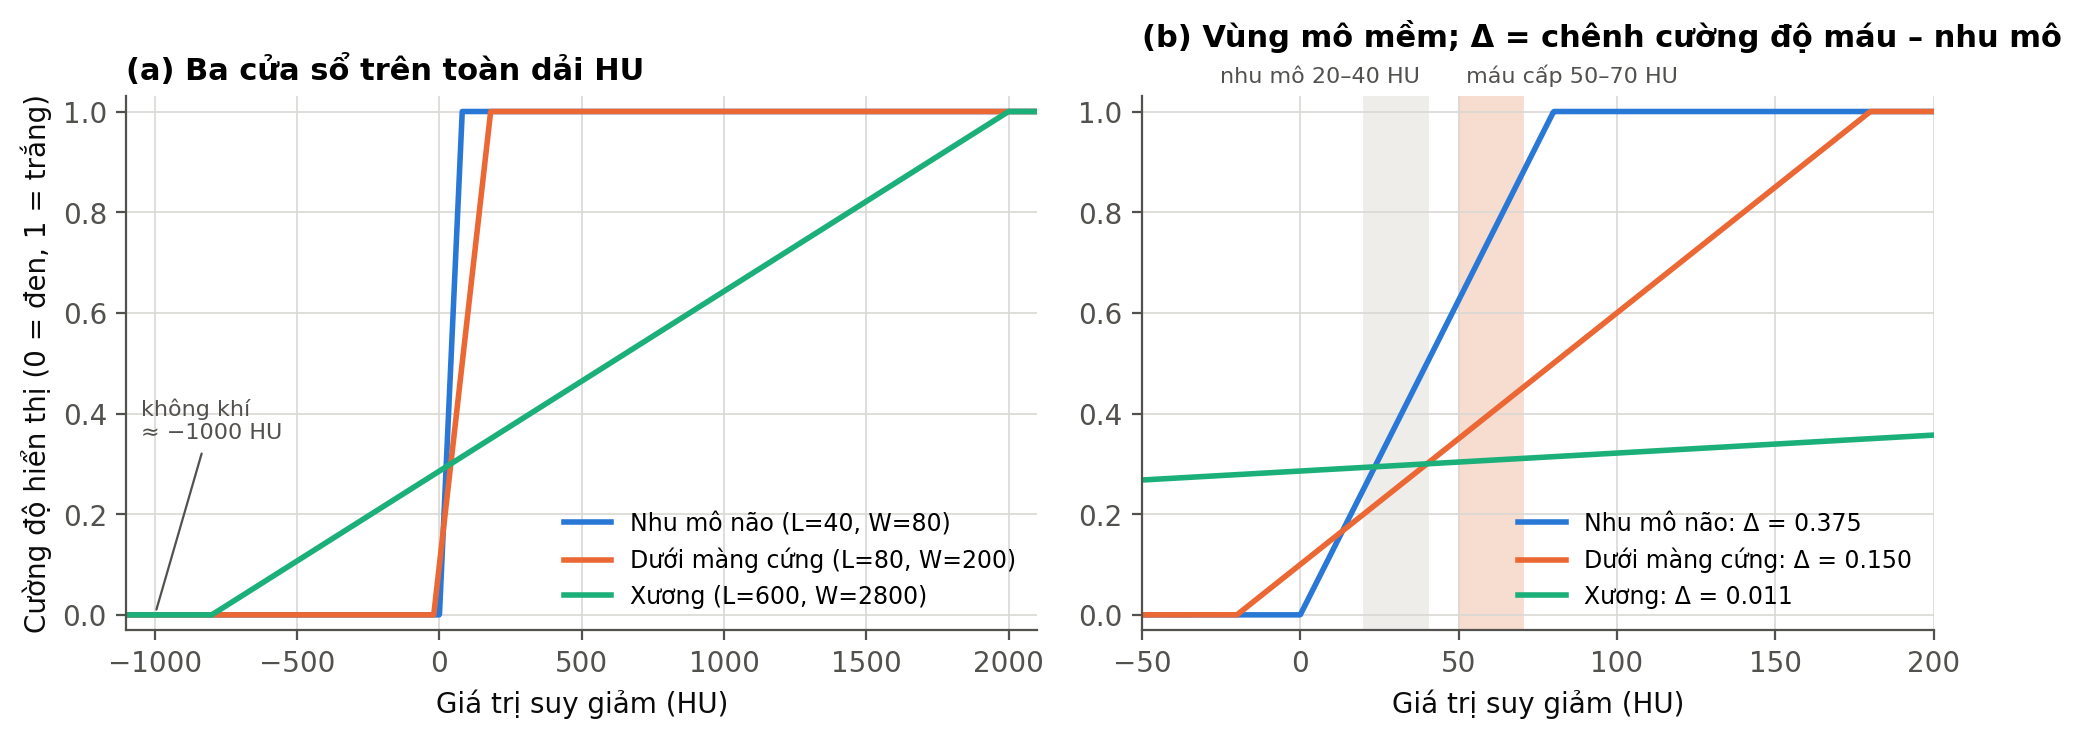
\includegraphics[width=\textwidth]{figures/fig_windowing.png}
\caption{Hàm ánh xạ cửa sổ hiển thị CT: (a) ba cửa sổ trên toàn dải HU; (b) phóng to
vùng mô mềm, với $\Delta$ là chênh lệch cường độ hiển thị giữa tâm vùng máu cấp
(60~HU) và tâm vùng nhu mô (30~HU). Mã nguồn: \texttt{figures/src/fig\_windowing.py}.}
\label{fig:windowing}
\end{figure}

Điều này dẫn tới một hệ quả kỹ thuật trực tiếp đối với cách lưu trữ dữ liệu. Vì
cửa sổ được chọn tuỳ theo điều bác sĩ đang tìm, hệ thống phải giữ nguyên dữ
liệu điểm ảnh DICOM gốc cùng các thuộc tính \texttt{RescaleSlope} và
\texttt{RescaleIntercept}, để trình xem có thể áp dụng bất kỳ cửa sổ nào tại
thời điểm đọc. Ngược lại, nếu lưu ảnh tám bit đã kết xuất sẵn thì quyết định
chọn cửa sổ đã được cố định một cách không thể đảo ngược, và bác sĩ mất khả
năng chuyển cửa sổ ngay trong lúc đọc.

\subsection{Quy trình lâm sàng và vai trò của nền tảng quản lý ảnh}

Một ca cấp tính điển hình diễn ra như sau. Bệnh nhân đến khoa cấp cứu; bác sĩ
chỉ định chụp CT sọ não; ca chụp được thực hiện trên thiết bị và truyền về
PACS; nó đi vào danh sách chờ đọc; một bác sĩ chẩn đoán hình ảnh đọc và ra kết
quả; bác sĩ điều trị xử trí dựa trên kết quả đó. Khoảng thời gian giữa lúc chụp
và lúc có kết quả chính là nơi độ trễ tích tụ, và một phần đáng kể độ trễ ấy
bắt nguồn từ khâu luân chuyển hình ảnh chứ không phải từ bản thân việc đọc.

Một nền tảng quản lý ảnh có thể rút ngắn chuỗi quy trình này ở những điểm sau:

\begin{itemize}
    \item \textbf{Truyền ảnh từ thiết bị về kho lưu trữ.} Ca chụp vừa hoàn tất
          được tự động chuyển về kho lưu trữ tập trung và sẵn sàng để đọc ngay,
          thay vì chờ thao tác thủ công tại máy trạm của thiết bị.
    \item \textbf{Truy cập hình ảnh từ nhiều vị trí.} Bác sĩ mở được ca chụp từ
          khoa phòng hoặc từ một máy tính bất kỳ trong bệnh viện, không nhất
          thiết phải có mặt tại phòng đọc chuyên dụng.
    \item \textbf{Đọc từ xa.} Khi cơ sở không có bác sĩ chẩn đoán hình ảnh tại
          chỗ, hình ảnh chuyển được tới bác sĩ ở nơi khác, điều này đặc biệt
          quan trọng ngoài giờ hành chính và ở tuyến dưới.
    \item \textbf{Loại bỏ khâu chuyển dữ liệu thủ công.} Việc ghi đĩa quang hay
          chép ổ đĩa di động để chuyển ảnh vừa chậm, vừa dễ thất lạc, vừa khó
          kiểm soát về mặt bảo mật.
\end{itemize}

Cần nhấn mạnh rằng nền tảng chỉ mang tính \emph{hỗ trợ}: nó cung cấp hình ảnh
và thông tin đi kèm một cách nhanh chóng và đầy đủ, chứ không đưa ra bất kỳ kết
luận nào. Chẩn đoán vẫn là hành vi của bác sĩ, phù hợp với quy định hành nghề
khám chữa bệnh của Việt Nam, theo đó chẩn đoán chỉ dành cho người có chứng chỉ
hành nghề. Do vậy, nền tảng phải được thiết kế sao cho mọi dữ liệu mà nó trình
bày đều truy được nguồn gốc và có thể đối chiếu lại với bản gốc.


\newpage
\section{DICOM và khả năng liên thông trong ảnh y khoa}
\label{sec:dicom}

Bất kỳ nền tảng nào muốn vận hành bên trong bệnh viện đều phải nói được ngôn ngữ
của bệnh viện. Đối với chẩn đoán hình ảnh, ngôn ngữ đó là DICOM, và các đặc tính
của nó ràng buộc kiến trúc hệ thống đủ nhiều để cần được trình bày như một nội
dung riêng thay vì chỉ là một chi tiết cài đặt.

\subsection{Chuẩn DICOM}

DICOM (Digital Imaging and Communications in Medicine, ISO 12052) là chuẩn quốc
tế quy định định dạng, lưu trữ và trao đổi ảnh y khoa \cite{dicom2024,pianykh2012dicom}. Chuẩn này bắt nguồn từ nỗ
lực của ACR--NEMA năm 1985 nhằm chấm dứt tình trạng phụ thuộc nhà cung cấp
(vendor lock-in) giữa các hãng sản xuất thiết bị chẩn đoán hình ảnh, và đã trở
nên phổ quát trên thực tế kể từ phiên bản 3.0 (1993). Điểm quan trọng là DICOM
không chỉ đơn thuần là một định dạng tệp. Nó đồng thời đặc tả:

\begin{itemize}
    \item một \textbf{mô hình thông tin} (information model), tổ chức dữ liệu
          theo phân cấp bốn mức Bệnh nhân $\rightarrow$ Ca chụp (Study)
          $\rightarrow$ Chuỗi ảnh (Series) $\rightarrow$ Đối tượng ảnh
          (Instance);
    \item một \textbf{định dạng tệp} trong đó dữ liệu điểm ảnh và siêu dữ liệu
          không thể tách rời, được mang trong cùng một đối tượng; và
    \item một họ \textbf{giao thức mạng} dùng để truy vấn, truy xuất và truyền
          tải các đối tượng đó.
\end{itemize}

Tính không thể tách rời giữa điểm ảnh và siêu dữ liệu là điểm xuất phát cho mọi
vấn đề tiếp theo. Một đối tượng DICOM là một chuỗi các \emph{phần tử dữ liệu}
(data element), mỗi phần tử được định danh bởi một \emph{thẻ} (tag), là cặp số
16 bit viết dưới dạng \texttt{(group,element)}. Bảng~\ref{tab:tags} liệt kê các
phần tử mà đề tài này phụ thuộc vào.

\begin{table}[H]
\centering
\small
\begin{tabularx}{\textwidth}{@{}l l X@{}}
\toprule
\textbf{Thẻ} & \textbf{Tên} & \textbf{Ý nghĩa} \\
\midrule
\texttt{(0010,0010)} & PatientName & Định danh trực tiếp; phải được loại bỏ trước khi dữ liệu rời khỏi bệnh viện \\
\texttt{(0010,0020)} & PatientID & Mã hồ sơ bệnh án của bệnh viện; định danh trực tiếp \\
\texttt{(0010,0030)} & PatientBirthDate & Bán định danh; có nguy cơ tái định danh khi kết hợp \\
\texttt{(0020,000D)} & StudyInstanceUID & Định danh duy nhất toàn cục của ca chụp; khóa chính của một ca chụp \\
\texttt{(0020,000E)} & SeriesInstanceUID & Định danh một chuỗi ảnh trong một ca chụp \\
\texttt{(0008,0018)} & SOPInstanceUID & Định danh một đối tượng ảnh đơn lẻ \\
\texttt{(0008,0050)} & AccessionNumber & Mã chỉ định do HIS/RIS cấp; khoá liên kết ca chụp với chỉ định và kết quả đọc (Mục~\ref{sec:his}) \\
\texttt{(0008,0060)} & Modality & \texttt{CT}, \texttt{MR}, \ldots; dùng để định tuyến \\
\texttt{(0028,1052)} & RescaleIntercept & Chuyển giá trị lưu trữ sang đơn vị Hounsfield \\
\texttt{(0028,1053)} & RescaleSlope & Chuyển giá trị lưu trữ sang đơn vị Hounsfield \\
\texttt{(0028,1050)} & WindowCenter & Cửa sổ hiển thị mặc định \\
\texttt{(0028,1051)} & WindowWidth & Cửa sổ hiển thị mặc định \\
\bottomrule
\end{tabularx}
\caption{Các phần tử dữ liệu DICOM mà nền tảng phụ thuộc vào.}
\label{tab:tags}
\end{table}

Giá trị điểm ảnh được lưu trữ bản thân chúng không phải là đơn vị Hounsfield;
phép chuyển đổi là

\begin{equation}
    \mathrm{HU} = \mathtt{RescaleSlope} \times p + \mathtt{RescaleIntercept},
    \label{eq:hu}
\end{equation}

trong đó $p$ là giá trị được lưu trữ. Áp dụng Công thức~\ref{eq:hu} trước mọi
thao tác cửa sổ là điều kiện để hình ảnh hiển thị nhất quán giữa các máy chụp
khác nhau và để các phép đo đậm độ có ý nghĩa so sánh được, bởi các nhà sản
xuất khác nhau dùng cách mã hóa giá trị lưu trữ khác nhau cho cùng một mức suy
giảm vật lý. Bỏ qua bước này thì cùng một mô, khi chụp trên hai thiết bị khác
hãng, sẽ hiển thị khác nhau trên trình xem.

\subsection{Các dịch vụ mạng}

Các thao tác mạng của DICOM được xây dựng trên các \emph{lớp dịch vụ} (service
class), trong đó một bên đóng vai trò Service Class User (SCU, bên yêu cầu) và
bên kia đóng vai trò Service Class Provider (SCP, bên đáp ứng). Các thao tác
liên quan ở đây gồm:

\begin{description}[leftmargin=2.2cm,style=nextline]
    \item[C-STORE] truyền một đối tượng ảnh từ nút này sang nút khác. Đây là cách
          máy chụp CT gửi một ca chụp đã hoàn tất tới PACS, và là điểm tự nhiên
          để nền tảng chặn bắt các ca chụp mới.
    \item[C-FIND] truy vấn các ca chụp thỏa mãn tiêu chí cho trước.
    \item[C-MOVE] yêu cầu một nút gửi các đối tượng ảnh phù hợp tới một bên thứ ba.
    \item[C-ECHO] kiểm tra kết nối, tương đương lệnh ping trong DICOM.
\end{description}

Các thao tác này chạy trên một liên kết TCP tại cổng thường được đánh số 104 hoặc
11112, và định danh các bên tham gia bằng \emph{Application Entity Title} (AE
Title), một tên ký hiệu ngắn. Việc thiết lập liên kết đòi hỏi mỗi bên phải nhận
biết AE Title của bên kia, qua đó cung cấp một cơ chế kiểm soát truy cập sơ khai:
một nút sẽ từ chối liên kết với một đối tác lạ. Đây là cấu hình chứ không phải
xác thực theo nghĩa mật mã học, và giao thức DICOM cổ điển mặc định truyền dữ
liệu ở dạng rõ. Do đó, mọi triển khai đi qua mạng không tin cậy đều phải bọc
DICOM trong TLS hoặc VPN, một yêu cầu sẽ xuất hiện trở lại ở
Mục~\ref{sec:architecture}.

\subsection{DICOMweb}

DICOMweb là cách diễn đạt lại các dịch vụ trên theo kiểu RESTful trên nền HTTP,
gồm WADO-RS (truy xuất), STOW-RS (lưu trữ) và QIDO-RS (truy vấn) \cite{dicomweb}. Nó quan trọng
với đề tài này vì một lý do thực tiễn: các trình xem chạy trên trình duyệt không
thể mở liên kết mạng DICOM thuần, nên một giao diện lâm sàng dạng web đòi hỏi
DICOMweb ở phía máy chủ. DICOMweb cũng kết hợp tự nhiên với hạ tầng HTTP thông
thường, bao gồm TLS, xác thực bằng bearer-token và reverse proxy, điều mà giao
thức cổ điển không làm được.

Bản mẫu của nền tảng phản ánh trực tiếp điều này. Orthanc, một PACS nhẹ mã nguồn
mở \cite{jodogne2018orthanc}, được cấu hình để đồng thời mở cổng DICOM cổ điển (4242) nhằm tiếp nhận ca
chụp từ các thiết bị và một giao diện DICOMweb (8042) cho trình xem, với reverse
proxy của trình xem chuyển tiếp \texttt{/dicom-web} và \texttt{/wado} tới đó.
Cách bố trí song giao thức này là điều cho phép một giao diện web hiện đại cùng
tồn tại với thiết bị chẩn đoán hình ảnh chỉ nói được giao thức năm 1993.

\subsection{Cú pháp truyền và nén ảnh}
\label{sec:transfersyntax}

Mỗi đối tượng DICOM được mã hoá theo một \emph{cú pháp truyền} (Transfer Syntax),
định danh bằng một UID, quy định thứ tự byte, cách biểu diễn kiểu dữ liệu và,
quan trọng nhất, cách nén dữ liệu điểm ảnh \cite{dicomps35}. Hai bên của một liên
kết DICOM thương lượng cú pháp truyền khi thiết lập liên kết; một nút không hỗ trợ
cú pháp của đối tác sẽ yêu cầu chuyển mã hoặc từ chối đối tượng. Bảng~\ref{tab:ts}
liệt kê các cú pháp liên quan tới đề tài.

\begin{table}[H]
\centering
\small
\begin{tabularx}{\textwidth}{@{}l l X@{}}
\toprule
\textbf{Cú pháp truyền} & \textbf{UID} & \textbf{Tính chất} \\
\midrule
Implicit VR Little Endian & \texttt{1.2.840.10008.1.2} & Mặc định bắt buộc phải hỗ trợ; không nén \\
Explicit VR Little Endian & \texttt{1.2.840.10008.1.2.1} & Không nén; phổ biến nhất \\
JPEG Lossless (SV1) & \texttt{1.2.840.10008.1.2.4.70} & Không mất mát; được thiết bị đời cũ hỗ trợ rộng rãi \\
JPEG-LS Lossless & \texttt{1.2.840.10008.1.2.4.80} & Không mất mát; nhanh, tỉ lệ nén tốt \\
JPEG 2000 (Lossless Only) & \texttt{1.2.840.10008.1.2.4.90} & Không mất mát; mở rộng được theo độ phân giải nhưng tốn tính toán khi giải mã \\
HTJ2K (Lossless Only) & \texttt{1.2.840.10008.1.2.4.201} & Bổ sung năm 2023 (Supplement 235); thông lượng mã hoá và giải mã cao \\
HTJ2K (Lossless RPCL) & \texttt{1.2.840.10008.1.2.4.202} & Như trên, sắp thứ tự luồng bit tối ưu cho hiển thị lũy tiến theo độ phân giải \\
HTJ2K & \texttt{1.2.840.10008.1.2.4.203} & Cho phép cả nén có mất mát lẫn không mất mát \\
\bottomrule
\end{tabularx}
\caption{Các cú pháp truyền DICOM liên quan tới nền tảng.}
\label{tab:ts}
\end{table}

Từ Mục~\ref{sec:windowing}, yêu cầu đối với nền tảng là rõ ràng: bản lưu trữ phục
vụ chẩn đoán chỉ được dùng cú pháp không mất mát. Nén có mất mát làm thay đổi giá
trị điểm ảnh, và vì phép cửa sổ khuếch đại các chênh lệch nhỏ về HU thành chênh
lệch lớn về cường độ hiển thị (Hình~\ref{fig:windowing}), sai số nén vốn khó thấy
trên ảnh thông thường có thể trở nên đáng kể khi đọc trong cửa sổ hẹp. Nén có mất
mát vì vậy chỉ được dùng cho ảnh thu nhỏ và ảnh xem trước. Với ảnh CT, nén không
mất mát thường chỉ giảm dung lượng vài lần, nhưng như vậy đã đủ thay đổi đáng kể
thời gian truyền qua đường truyền chậm (Hình~\ref{fig:transfer}) và dung lượng
lưu trữ dài hạn (Hình~\ref{fig:storage}).

Trong nhóm không mất mát, HTJ2K \cite{dicomsup235} đáng được chú ý vì hai lý do.
Thứ nhất, nó giữ các tính năng của JPEG 2000, như khả năng mở rộng theo độ phân
giải, nhưng thay bộ mã hoá khối bằng một thuật toán có thông lượng cao hơn đáng
kể, loại bỏ nhược điểm chính khiến JPEG 2000 ít được dùng trong hiển thị thời gian
thực. Thứ hai, với biến thể RPCL, trình xem có thể hiển thị một phiên bản độ phân
giải thấp của lát cắt ngay khi nhận được phần đầu của luồng bit và làm nét dần khi
phần còn lại đến. Cornerstone3D, lớp hiển thị của OHIF từ phiên bản 3, hỗ trợ kiểu
tải lũy tiến này, và dịch vụ AWS HealthImaging cũng lưu dữ liệu điểm ảnh dưới dạng
HTJ2K \cite{awshealthimaging}. Với đường truyền chậm ở bối cảnh C, đây là cơ chế
cho phép bác sĩ tuyến trên bắt đầu đọc trước khi toàn bộ ca chụp được truyền xong;
mức lợi ích thực tế cần được đo trong Giai đoạn~2.

\subsection{Tích hợp với hệ thống thông tin bệnh viện}
\label{sec:his}

Ảnh chụp chỉ có ý nghĩa lâm sàng khi gắn với đúng bệnh nhân, đúng chỉ định và đúng
kết quả đọc. Những thông tin này nằm trong hệ thống thông tin bệnh viện (HIS), hệ
thống thông tin chẩn đoán hình ảnh (RIS) và hồ sơ bệnh án điện tử (EMR), không nằm
trong PACS. Một nền tảng quản lý ảnh vì vậy phải trao đổi với các hệ thống đó qua
các cơ chế chuẩn sau.

\begin{description}[leftmargin=2.6cm,style=nextline]
\item[Modality Worklist] Thiết bị chụp truy vấn danh sách ca đã được chỉ định
      (C-FIND trên worklist) để lấy thông tin bệnh nhân, mã chỉ định
      (\texttt{AccessionNumber}) và thủ thuật cần chụp, thay vì kỹ thuật viên
      nhập tay. Đây là biện pháp hiệu quả nhất để tránh sai lệch định danh ngay
      từ nguồn. Modality Performed Procedure Step (MPPS) báo ngược trạng thái
      đã chụp.
\item[HL7 v2] Chuẩn nhắn tin vẫn phổ biến nhất giữa HIS và RIS: bản tin ADT cho
      thông tin hành chính của bệnh nhân, ORM/OMI cho chỉ định, ORU cho kết
      quả.
\item[HL7 FHIR] Chuẩn REST hiện đại. Các tài nguyên liên quan gồm
      \texttt{Patient}, \texttt{ServiceRequest}, \texttt{ImagingStudy} (tham
      chiếu tới ca chụp qua StudyInstanceUID và điểm truy cập DICOMweb) và
      \texttt{DiagnosticReport} \cite{hl7fhir}. FHIR phù hợp cho các hệ thống
      mới và cho trao đổi liên viện.
\item[Hồ sơ IHE] IHE không định nghĩa chuẩn mới mà quy định cách phối hợp các
      chuẩn trên trong từng kịch bản. Liên quan trực tiếp là Scheduled
      Workflow (SWF.b) cho luồng chỉ định--chụp--đọc, Patient Information
      Reconciliation (PIR) cho việc sửa định danh sau khi đã chụp, XDS-I.b cho
      chia sẻ ảnh giữa các cơ sở \cite{iherad}, và Audit Trail and Node
      Authentication (ATNA) cho xác thực nút mạng bằng TLS và định dạng bản ghi
      nhật ký truy vết \cite{iheiti}.
\end{description}

Mức độ tích hợp khả thi phụ thuộc bối cảnh. Ở bối cảnh A, HIS/RIS thường đã hỗ
trợ HL7 và worklist, và nền tảng chỉ cần nhận bản tin. Ở bối cảnh C, thường không
có RIS, worklist không khả dụng và định danh được nhập tay trên máy chụp; nền tảng
phải chấp nhận thực tế này và cung cấp chức năng đối chiếu, sửa định danh có ghi
nhật ký theo tinh thần PIR. Ngoài ra, Thông tư 13/2025/TT-BYT yêu cầu hồ sơ bệnh
án điện tử kết nối với cơ sở dữ liệu quốc gia về dân cư (Mục~\ref{sec:legal}); khi
đó số định danh cá nhân trở thành khoá liên kết bệnh nhân giữa các cơ sở, đồng thời
là một định danh trực tiếp phải bị loại bỏ khi khử định danh.

\subsection{Khử định danh}
\label{sec:deid}

Vì các định danh được nhúng ngay trong bản thân đối tượng ảnh, việc chia sẻ một
đối tượng DICOM đồng nghĩa với chia sẻ danh tính bệnh nhân, trừ khi có hành động
chủ động ngăn chặn. DICOM PS3.15 Phụ lục E \cite{dicomps315} định nghĩa các Hồ sơ bảo mật
(Confidentiality Profile) quy định thuộc tính nào phải bị loại bỏ, thay thế hoặc
giữ lại tùy theo mục đích sử dụng.

Ba khó khăn thường tái diễn trong thực tế và phải được xử lý tường minh:

\begin{enumerate}
    \item \textbf{Chú thích in chìm vào ảnh.} Một số thiết bị vẽ thông tin bệnh
          nhân trực tiếp vào mảng điểm ảnh. Thuộc tính
          \texttt{(0028,0301) BurnedInAnnotation} báo hiệu điều này nhưng không
          được điền nhất quán, nên có thể cần kiểm tra ở mức điểm ảnh.
    \item \textbf{Thẻ riêng của nhà sản xuất.} Các hãng lưu dữ liệu độc quyền
          trong những nhóm thẻ riêng với ngữ nghĩa không được công bố. Chính sách
          an toàn là loại bỏ toàn bộ thẻ riêng, chấp nhận mất các tham số thu
          nhận ảnh mà chúng mang theo.
    \item \textbf{Tính nhất quán của UID.} Thay thế UID một cách ngẫu nhiên sẽ
          phá vỡ quan hệ ca chụp--chuỗi ảnh--đối tượng ảnh. Khử định danh phải áp
          dụng một phép ánh xạ đơn ánh nhất quán để giữ nguyên cấu trúc phân cấp
          trong khi các định danh gốc không thể khôi phục được.
\end{enumerate}

Hơn nữa, khử định danh cần được hiểu là giảm thiểu rủi ro chứ không phải loại bỏ
rủi ro. Ảnh CT sọ não chứa cấu trúc khuôn mặt của bệnh nhân, và việc dựng bề mặt
từ một khối ảnh đã khử định danh có thể tạo ra một khuôn mặt nhận diện được; khả
năng này đã được ghi nhận trong y văn \cite{schwarz2019identification} và có nghĩa là dữ liệu hình ảnh phải được
đối xử như dữ liệu cá nhân ngay cả sau khi đã loại bỏ các thẻ. Giá trị pháp lý
của kết luận này theo pháp luật Việt Nam được bàn luận ở Mục~\ref{sec:legal}.


\newpage
\section{Khảo sát các giải pháp phần mềm hiện có}
\label{sec:solutions}

\subsection{Các hệ thống PACS/VNA thương mại}

Thị trường phần mềm quản lý và lưu trữ ảnh y khoa từ lâu do một số nhà cung cấp
lớn chi phối. GE Healthcare, Siemens Healthineers và Philips đều phát triển các
hệ thống PACS gắn liền với dòng thiết bị chẩn đoán hình ảnh của chính mình.
Fujifilm với dòng sản phẩm Synapse, cùng Sectra và Agfa HealthCare, cung cấp các
nền tảng PACS và VNA hướng tới quy mô bệnh viện và mạng lưới nhiều cơ sở.

Điểm chung của nhóm này là mức độ hoàn chỉnh cao. Hệ thống được cung cấp trọn
gói, kèm dịch vụ triển khai, đào tạo và bảo trì, tích hợp sẵn với HIS và RIS
theo các chuẩn HL7 và DICOM, đồng thời phối hợp chặt chẽ với máy chụp cùng hãng.
Đổi lại, chi phí đầu tư và phí duy trì hằng năm ở mức cao, mã nguồn đóng và cấu
trúc dữ liệu nội bộ thường không được công bố, khiến cơ sở y tế rơi vào tình
trạng phụ thuộc nhà cung cấp cả về nâng cấp, mở rộng lẫn di chuyển dữ liệu về
sau.

\subsection{Các hệ thống PACS mã nguồn mở}

\textbf{Orthanc} là một PACS mã nguồn mở nhẹ với giấy phép thoáng. Hệ thống chạy
từ một tệp nhị phân duy nhất, không bắt buộc phải có cơ sở dữ liệu bên ngoài, hỗ
trợ đồng thời giao thức DICOM cổ điển và DICOMweb, đồng thời tích hợp bộ thông
dịch Lua cho phép định nghĩa các hành vi tự động khi có ảnh mới đến. Nhờ yêu cầu
tài nguyên thấp, Orthanc phù hợp cả khi đóng vai trò PACS đầy đủ tại một cơ sở
nhỏ lẫn khi làm cổng tích hợp đặt cạnh một PACS sẵn có tại cơ sở lớn
\cite{jodogne2018orthanc}.

Điểm đáng chú ý của Orthanc là hệ sinh thái plugin, cho phép bổ sung đúng những
năng lực mà lõi còn thiếu mà không phải sửa lõi \cite{orthancbook}. Plugin
PostgreSQL thay SQLite mặc định bằng một cơ sở dữ liệu chịu tải cao làm chỉ mục, và
cho phép nhiều phiên bản Orthanc dùng chung chỉ mục. Plugin lưu trữ đối tượng ghi
dữ liệu điểm ảnh lên kho tương thích S3, Azure Blob hoặc Google Cloud Storage thay
vì hệ thống tệp cục bộ. Plugin DICOMweb cung cấp WADO-RS, STOW-RS và QIDO-RS. Plugin
phân quyền nâng cao chuyển mọi quyết định cấp quyền cho một dịch vụ web bên ngoài,
và dự án orthanc-auth-service hiện thực sẵn dịch vụ này trên nền máy chủ định danh
Keycloak, kèm cơ chế chia sẻ ca chụp bằng token \cite{orthancauth,keycloak}. Tổ hợp
này giải quyết được một phần đáng kể các điểm yếu về quản trị nêu ở
Mục~\ref{sec:solutions-analysis}, nhưng vẫn là việc lắp ghép cần được thiết kế và
kiểm thử.

\textbf{dcm4che} là bộ công cụ DICOM viết bằng Java, đã trưởng thành qua nhiều
năm phát triển và được xem là một trong những hiện thực DICOM mã nguồn mở đầy đủ
nhất. Trên nền bộ công cụ này, \textbf{dcm4chee-arc} cung cấp một kho lưu trữ ảnh
ở quy mô doanh nghiệp, hỗ trợ phong phú các dịch vụ DICOM và DICOMweb cùng các
cơ chế quản trị dữ liệu. Bù lại, hệ thống đòi hỏi hạ tầng nặng hơn đáng kể, gồm
máy chủ ứng dụng Java và cơ sở dữ liệu riêng, cũng như nhân sự quen thuộc với hệ
sinh thái Java.

\subsection{Các trình xem ảnh y khoa}

\textbf{OHIF Viewer}, do Open Health Imaging Foundation duy trì \cite{ziegler2020ohif}, là trình xem mã
nguồn mở chạy hoàn toàn trên trình duyệt. Đặc tính không cần cài đặt tại máy
trạm (zero-footprint) giúp loại bỏ khâu triển khai và cập nhật phần mềm trên
từng máy tính, một lợi thế rõ rệt tại các cơ sở có năng lực quản trị công nghệ
thông tin hạn chế. Kiến trúc mở rộng theo mô-đun cho phép bổ sung công cụ đo
đạc, bố cục hiển thị hay lớp phủ thông tin ngay trong giao diện đọc ảnh tiêu
chuẩn. Từ phiên bản 3, OHIF dựa trên Cornerstone3D, hỗ trợ dựng hình bằng GPU và tải
ảnh lũy tiến (Mục~\ref{sec:transfersyntax}).

\textbf{Cornerstone.js} là thư viện hiển thị ảnh y khoa trên nền web, đảm nhận
việc giải mã, dựng hình và tương tác với dữ liệu DICOM. Đây chính là lớp nền mà
OHIF Viewer xây dựng bên trên, và cũng có thể được dùng trực tiếp khi cần một
giao diện xem ảnh gọn nhẹ, gắn chặt với ứng dụng sẵn có.

\textbf{Weasis} là trình xem chạy trên máy trạm, viết bằng Java, hỗ trợ nhiều
phương thức chụp và có thể khởi chạy trực tiếp từ liên kết do PACS sinh ra. Ưu
điểm của trình xem desktop là khai thác tốt tài nguyên máy cục bộ, nhưng đi kèm
với đó là yêu cầu cài đặt và duy trì phần mềm trên từng máy.

\subsection{Các thành phần mã nguồn mở chuyên biệt}

Ngoài PACS và trình xem, một số dự án mã nguồn mở giải quyết đúng từng khâu mà
đề tài cần, và là tham chiếu trực tiếp cho thiết kế ở Mục~\ref{sec:architecture}.

\textbf{KHEOPS} là nền tảng chia sẻ ảnh DICOM, tổ chức ca chụp theo ``album'' và
cấp quyền truy cập bằng token gắn với một album hoặc một ca chụp, có thể giới hạn
quyền và thời hạn; dữ liệu được truy cập qua DICOMweb và mở bằng OHIF hoặc Weasis
\cite{kheops}. Mô hình token phạm vi hẹp này khớp với kịch bản gửi một ca chụp cho
bác sĩ tuyến trên mà không cấp cho họ quyền vào toàn bộ kho ảnh.

\textbf{Karnak}, của cùng nhóm phát triển, là cổng DICOM chuyên khử định danh và
định tuyến ảnh theo các hồ sơ của DICOM PS3.15, với giao diện cấu hình quy tắc khử
định danh cho từng dự án \cite{karnak}. Đây là tham chiếu cho khâu khử định danh
tại ranh giới của bộ điều phối.

\textbf{MONAI Deploy Informatics Gateway} tiếp nhận dữ liệu qua DICOM DIMSE,
DICOMweb và FHIR, gom các đối tượng thành ca chụp, phát sự kiện kích hoạt quy trình
xử lý và gửi kết quả ngược về PACS \cite{monaiig}. Về chức năng, nó gần như trùng
với bộ điều phối trong mô hình thành phần, và là ứng viên nên được đánh giá trước
khi tự xây dựng, đặc biệt khi các thành phần phân tích ảnh tự động được bổ sung ở
các giai đoạn sau. Đổi lại, nó cần thêm hàng đợi thông điệp và kho đối tượng, nặng
so với thiết bị trọn gói ở bối cảnh C.

\subsection{Các nền tảng ảnh y khoa trên đám mây}
\label{sec:cloud}

Các nhà cung cấp đám mây lớn đều có dịch vụ quản lý ảnh y khoa: AWS HealthImaging
\cite{awshealthimaging}, kho DICOM của Google Cloud Healthcare API
\cite{gcphealthcare}, và dịch vụ DICOM của Azure Health Data Services, vốn phát
triển từ dự án mã nguồn mở Medical Imaging Server for DICOM của Microsoft
\cite{msdicom}. Cả ba đều cung cấp DICOMweb, tự mở rộng quy mô và tính phí theo
dung lượng và lưu lượng. Chúng thay thế tầng lưu trữ, không thay thế trình xem
hay quy trình đọc ảnh.

Bài viết của AWS về xây dựng PACS gốc đám mây \cite{awspacs2026} đáng được phân
tích kỹ vì nó đi tới cùng kết luận với đề tài từ hướng ngược lại. Kiến trúc được đề
xuất là mô hình lai trục--nan: mỗi bệnh viện giữ một máy chủ VNA cục bộ tiếp nhận
ảnh qua C-STORE và phục vụ bác sĩ tại chỗ ở tốc độ mạng nội bộ, còn ảnh được sao
chép bất đồng bộ lên kho đối tượng trung tâm qua kênh riêng mà không chặn luồng lâm
sàng. Một cơ sở dữ liệu trung tâm chỉ chứa siêu dữ liệu, gồm chỉ mục bệnh nhân
chung, vị trí của từng ca chụp và trạng thái đồng bộ, cho phép bác sĩ ở bệnh viện
này tìm và mở ca chụp thực hiện ở bệnh viện khác; trình xem tự định tuyến yêu cầu
tới bản cục bộ nếu còn trong bộ đệm, hoặc tới kho trung tâm nếu không. Bài viết
dựa trên quan sát rằng tần suất truy cập ảnh cao trong vài tháng đầu, giảm mạnh sau
6--12 tháng và hiếm khi được truy cập sau 2--3 năm để đề xuất phân tầng lưu trữ theo
vòng đời, từ lớp truy cập thường xuyên tới lớp lưu trữ sâu cho dữ liệu trên năm năm,
và khuyến nghị mô hình lai thay vì thuần đám mây khi kết nối mạng hạn chế hoặc chỉ
phụ thuộc một nhà mạng.

Đối chiếu với đề tài: (i) nguyên tắc ghi cục bộ trước, đồng bộ sau
(Mục~\ref{sec:localfirst}) trùng khớp, cho thấy đây không chỉ là lựa chọn bắt buộc
của cơ sở thiếu tài nguyên mà còn là thực hành được khuyến nghị ở quy mô lớn; (ii)
tách chỉ mục khỏi điểm ảnh và phân tầng theo vòng đời là hai điểm đề tài tiếp thu,
trình bày ở Mục~\ref{sec:tiering} và Mục~\ref{sec:hub}; (iii) khác biệt nằm ở giả
định. Bài viết giả định kênh kết nối riêng ổn định, đội ngũ vận hành, và khả năng đặt
dữ liệu tại một vùng đám mây trong lãnh thổ quốc gia; ở Việt Nam, dữ liệu đưa ra
ngoài lãnh thổ phải qua đánh giá tác động chuyển dữ liệu xuyên biên giới
(Mục~\ref{sec:legal}), và ở bối cảnh C kênh kết nối chính là điểm yếu nhất. Vì vậy
đề tài đặt trung tâm ở hạ tầng trong nước và chỉ gửi ra ngoài bệnh viện bản sao lưu
đã mã hoá và bản đã khử định danh.


\subsection{Bối cảnh trong nước}

Tại Việt Nam, chủ trương chuyển đổi số ngành y tế và lộ trình triển khai bệnh án
điện tử đang thúc đẩy các bệnh viện thay thế phim in bằng hệ thống lưu trữ và
truyền tải hình ảnh. Thông tư 13/2025/TT-BYT đặt thời hạn triển khai hồ sơ bệnh án
điện tử cho các bệnh viện chậm nhất ngày 30/9/2025 và cho các cơ sở khám bệnh, chữa
bệnh khác chậm nhất ngày 31/12/2026 \cite{tt13_2025}; vì kết quả cận lâm sàng, trong
đó có chẩn đoán hình ảnh, là một phần của hồ sơ bệnh án, lộ trình này tạo áp lực
trực tiếp lên việc số hoá và lưu trữ ảnh ở chính nhóm cơ sở chưa có PACS. Nhiều cơ sở lớn lựa chọn giải pháp thương mại nhập khẩu
hoặc dịch vụ do doanh nghiệp trong nước cung cấp, trong khi tuyến huyện và các
phòng khám phần lớn vẫn gặp trở ngại về chi phí đầu tư và nhân lực vận hành. Đây
là khoảng trống mà một giải pháp xây dựng trên nền tảng mã nguồn mở có thể lấp
đầy.

\section{Phân tích các giải pháp hiện có}
\label{sec:solutions-analysis}

\subsection{Điểm mạnh}

Các hệ thống PACS thương mại mang lại sự hoàn chỉnh và tính ổn định đã được kiểm
chứng qua nhiều năm vận hành lâm sàng. Người mua nhận được một sản phẩm trọn gói
cùng cam kết hỗ trợ kỹ thuật, quy trình tích hợp với HIS và RIS đã được chuẩn
hoá, và trách nhiệm khắc phục sự cố thuộc về một đầu mối duy nhất. Với bệnh viện
có lưu lượng chụp lớn và ngân sách tương xứng, đây là phương án giảm thiểu rủi ro
triển khai.

Nhóm mã nguồn mở lại mạnh ở những khía cạnh khác. Chi phí cấp phép gần như bằng
không cho phép dồn nguồn lực vào hạ tầng và con người thay vì bản quyền phần mềm.
Mã nguồn công khai giúp kiểm tra được cách dữ liệu được lưu trữ và xử lý, đồng
thời cho phép tuỳ biến sâu theo quy trình thực tế của từng khoa chẩn đoán hình
ảnh. Việc tuân thủ chặt các chuẩn DICOM và DICOMweb giữ cho dữ liệu luôn ở định
dạng mở, nhờ đó có thể chuyển đổi giữa các hệ thống mà không bị ràng buộc. Riêng
Orthanc và OHIF còn nổi bật ở yêu cầu tài nguyên thấp, đủ để vận hành trên một
máy chủ phổ thông tại cơ sở tuyến dưới.

\subsection{Điểm yếu và khoảng trống}

\textbf{Chi phí và cấp phép.} Các hệ thống thương mại được định giá cho những
bệnh viện dồi dào ngân sách, theo hình thức mua bản quyền kèm phí bảo trì hằng
năm hoặc tính theo dung lượng lưu trữ. Với bệnh viện tuyến huyện và phòng khám
tư nhân quy mô nhỏ, mức chi phí này vượt quá khả năng chi trả, trong khi đây lại
chính là nhóm cơ sở cần một hệ thống quản lý ảnh có tổ chức nhất.

\textbf{Phụ thuộc nhà cung cấp.} Khi hệ thống đóng kín và cấu trúc lưu trữ không
được công bố, mọi thay đổi về sau đều phải đi qua nhà cung cấp ban đầu. Việc mở
rộng thêm chức năng, kết nối với hệ thống của bên thứ ba hay di chuyển toàn bộ
kho ảnh sang nền tảng khác đều trở nên tốn kém, và cơ sở y tế mất phần lớn quyền
chủ động đối với hạ tầng của chính mình.

\textbf{Khả năng tuỳ biến.} Quy trình làm việc tại mỗi khoa chẩn đoán hình ảnh
có những khác biệt nhất định, từ cách phân luồng ca chụp đến biểu mẫu kết quả.
Sản phẩm thương mại chỉ cho phép cấu hình trong khuôn khổ nhà sản xuất định sẵn,
còn những yêu cầu nằm ngoài khuôn khổ đó thường phải chờ bản cập nhật hoặc trả
phí phát triển riêng.

\textbf{Hạ tầng và nhân lực vận hành.} Ở chiều ngược lại, các giải pháp mã nguồn
mở quy mô doanh nghiệp như dcm4chee-arc đòi hỏi đội ngũ có kinh nghiệm quản trị
máy chủ, cơ sở dữ liệu và mạng. Nhiều cơ sở tuyến dưới không có sẵn nhân lực như
vậy, nên một hệ thống tuy miễn phí nhưng phức tạp vẫn có thể trở thành gánh nặng
vận hành.

\textbf{Triển khai tại cơ sở hạn chế tài nguyên.} Phần lớn giải pháp thương mại
mặc định rằng cơ sở đã có máy chủ đủ mạnh, đường truyền ổn định và bộ phận công
nghệ thông tin thường trực. Những nơi không đáp ứng được các điều kiện đó gần
như không có phương án phù hợp, và khả năng vận hành ở chế độ hạn chế khi mạng
gián đoạn hiếm khi được tính đến.

\textbf{Chủ quyền dữ liệu.} Các dịch vụ lưu trữ ảnh trên đám mây đòi hỏi dữ liệu
hình ảnh rời khỏi phạm vi cơ sở y tế, làm phát sinh những ràng buộc mà
Mục~\ref{sec:legal} cho thấy không đơn thuần mang tính hợp đồng theo pháp luật
Việt Nam. Khả năng lưu trữ và xử lý hoàn toàn tại chỗ vì vậy là một yêu cầu
thực chất chứ không phải tuỳ chọn.

\textbf{Gánh nặng tích hợp của các thành phần mã nguồn mở.} Hệ sinh thái mã
nguồn mở tránh được chi phí cấp phép nhưng chỉ cung cấp các thành phần rời rạc,
không phải một giải pháp hoàn chỉnh. Orthanc, OHIF và các thư viện liên quan,
xét riêng từng thành phần, đều đã trưởng thành; nhưng ghép chúng thành một hệ
thống có xác thực người dùng, phân quyền theo vai trò, nhật ký kiểm toán, giám
sát và hành vi được định nghĩa rõ ràng khi xảy ra sự cố là một khối lượng công
việc kỹ thuật đáng kể. Chính phần lắp ghép này tạo nên đóng góp của đề tài.

\begin{table}[H]
\centering
\small
\begin{tabularx}{\textwidth}{@{}X X X@{}}
\toprule
\textbf{Giải pháp} & \textbf{Điểm mạnh} & \textbf{Điểm yếu} \\
\midrule
PACS thương mại (GE, Siemens, Philips, Fujifilm, Sectra, Agfa) & Hoàn chỉnh; hỗ trợ chính hãng; tích hợp sâu với thiết bị và với HIS/RIS & Chi phí đầu tư và duy trì cao; mã nguồn đóng; phụ thuộc nhà cung cấp; khó tuỳ biến \\
Orthanc & Nhẹ, một tệp nhị phân; hỗ trợ cả DICOM cổ điển lẫn DICOMweb; scripting Lua; giấy phép thoáng & Thiếu sẵn các chức năng quản trị cấp bệnh viện; phải tự bổ sung xác thực, phân quyền và giám sát \\
dcm4che/dcm4chee-arc & Trưởng thành; đầy đủ dịch vụ DICOM; phù hợp quy mô doanh nghiệp & Hạ tầng nặng; cấu hình phức tạp; đòi hỏi nhân lực quản trị Java và cơ sở dữ liệu \\
OHIF Viewer & Chạy trên trình duyệt, không cần cài đặt tại máy trạm; kiến trúc mở rộng theo mô-đun & Phụ thuộc năng lực máy khách và đường truyền; cần tuỳ biến để khớp quy trình đọc ảnh cụ thể \\
Weasis & Trình xem desktop giàu chức năng; khai thác tốt tài nguyên máy cục bộ & Phải cài đặt và cập nhật trên từng máy trạm \\
Cornerstone.js & Thư viện hiển thị linh hoạt, nhúng được vào ứng dụng web sẵn có & Chỉ là thư viện, không phải trình xem hoàn chỉnh; phải tự xây dựng giao diện \\
Plugin Orthanc (PostgreSQL, lưu trữ đối tượng, phân quyền) & Bổ sung chỉ mục chịu tải, lưu trữ S3, phân quyền qua Keycloak mà không sửa lõi & Mỗi plugin là một điểm cấu hình và nâng cấp riêng; cần kiểm thử tổ hợp \\
KHEOPS & Chia sẻ ca chụp bằng token phạm vi hẹp; DICOMweb; tích hợp OHIF và Weasis & Thêm một hệ thống cần vận hành; không tiếp nhận trực tiếp từ máy chụp \\
Karnak & Khử định danh theo hồ sơ PS3.15, cấu hình qua giao diện & Chỉ giải quyết khâu khử định danh và định tuyến \\
MONAI Deploy Informatics Gateway & Tiếp nhận DIMSE, DICOMweb, FHIR; phát sự kiện; trả kết quả về PACS & Hướng tới quy trình AI; phụ thuộc hàng đợi thông điệp và kho đối tượng \\
Dịch vụ đám mây (AWS HealthImaging, Google Cloud Healthcare API, Azure DICOM) & Không phải vận hành hạ tầng lưu trữ; tự mở rộng; DICOMweb & Dữ liệu rời khỏi bệnh viện; ràng buộc chuyển dữ liệu xuyên biên giới; phụ thuộc đường truyền và nhà cung cấp \\
\bottomrule
\end{tabularx}
\caption{Phân tích so sánh các giải pháp quản lý và hiển thị ảnh y khoa hiện có.}
\label{tab:solutions}
\end{table}


\newpage
\section{Khung pháp lý về bảo vệ dữ liệu bệnh nhân tại Việt Nam}
\label{sec:legal}

Hình ảnh y tế là dữ liệu cá nhân thuộc nhóm nhạy cảm nhất, và tại Việt Nam việc
xử lý loại dữ liệu này chịu sự điều chỉnh của một khung pháp lý nhiều tầng gồm
pháp luật chuyên ngành y tế, pháp luật chung về bảo vệ dữ liệu cá nhân và pháp
luật về an ninh mạng. Các ràng buộc này mang tính kiến trúc: chúng quyết định
dữ liệu được lưu trú ở đâu, ai được phép truy cập và những gì bắt buộc phải ghi
nhận, và không thể bổ sung thêm về sau vào một hệ thống vốn được thiết kế mà
không tính đến chúng.

\subsection{Pháp luật chuyên ngành y tế}

\textbf{Luật Khám bệnh, chữa bệnh} (số 15/2023/QH15, có hiệu lực từ ngày 01
tháng 01 năm 2024) \cite{lawmet2023} xác lập quyền được bảo mật thông tin của người bệnh như một
quyền luật định. Thông tin về tình trạng sức khoẻ và đời tư của người bệnh được
ghi trong hồ sơ bệnh án phải được giữ bí mật và chỉ được tiết lộ khi có sự đồng
ý của người bệnh hoặc trong các trường hợp pháp luật cho phép. Cũng chính luật
này điều chỉnh bản thân hồ sơ bệnh án, quy định thời hạn lưu trữ và xác định
những chủ thể được phép tiếp cận, đồng thời khẳng định chẩn đoán là hoạt động
chỉ dành cho người hành nghề có giấy phép. Điểm cuối cùng này là cơ sở pháp lý
cho định hướng hỗ trợ được giữ nhất quán trong toàn bộ báo cáo: nền tảng có thể
cung cấp thông tin phục vụ chẩn đoán nhưng không được đưa ra chẩn đoán.

\textbf{Thông tư 13/2025/TT-BYT} hướng dẫn triển khai hồ sơ bệnh án điện tử
(ban hành ngày 06/6/2025, có hiệu lực từ ngày 21/7/2025) thay thế Thông tư
46/2018/TT-BYT \cite{tt13_2025,mohemr}. Thông tư đặt lộ trình bắt buộc: các bệnh
viện phải triển khai chậm nhất ngày 30/9/2025, các cơ sở khám bệnh, chữa bệnh khác
chậm nhất ngày 31/12/2026. Cơ sở phải có hạ tầng gồm máy chủ, thiết bị lưu trữ,
giải pháp an toàn thông tin và phần mềm quản lý hồ sơ; hệ thống phải đáp ứng tiêu
chuẩn kỹ thuật về an toàn thông tin và có khả năng phục hồi dữ liệu, hỗ trợ chữ ký
số hoặc phương thức xác thực hợp pháp khác, và kết nối với cơ sở dữ liệu quốc gia
về dân cư. Hai yêu cầu có hệ quả kiến trúc trực tiếp. Yêu cầu truy xuất và kiểm tra
hồ sơ về sau khiến một nhật ký truy vết chỉ ghi thêm (append-only), ghi nhận mọi
truy cập, trở thành yêu cầu chức năng chứ không còn là lựa chọn thiết kế. Yêu cầu
khả năng phục hồi dữ liệu biến độ bền của kho ảnh thành nghĩa vụ pháp lý, không
chỉ là chất lượng kỹ thuật.

\subsection{Bảo vệ dữ liệu cá nhân}

Khung bảo vệ dữ liệu cá nhân của Việt Nam đã thay đổi căn bản trong thời gian
thực hiện đề tài. \textbf{Nghị định 13/2023/NĐ-CP}, có hiệu lực từ ngày 01/7/2023,
là văn bản toàn diện đầu tiên \cite{decree13}. Kể từ ngày 01/01/2026, vai trò này
thuộc về \textbf{Luật Bảo vệ dữ liệu cá nhân số 91/2025/QH15}, được Quốc hội thông
qua ngày 26/6/2025, cùng \textbf{Nghị định 356/2025/NĐ-CP} quy định chi tiết thi
hành, thay thế Nghị định 13 \cite{pdpl2025,decree356}. Các hồ sơ đánh giá tác động
đã lập theo Nghị định 13 vẫn được công nhận, nhưng mọi cập nhật về sau phải tuân
theo luật mới. Phần lớn nghĩa vụ được kế thừa từ Nghị định 13, nay được nâng lên
tầm luật và đi kèm chế tài nặng hơn. Một số quy định tác động trực tiếp đến thiết
kế hệ thống.

Luật phân biệt \emph{dữ liệu cá nhân cơ bản} với \emph{dữ liệu cá nhân nhạy cảm}
và xếp thông tin về tình trạng sức khoẻ vào nhóm nhạy cảm, kéo theo các nghĩa vụ
tăng cường. Sự đồng ý phải tự nguyện, rõ ràng và cụ thể cho từng mục đích; sự im
lặng không được coi là đồng ý, và chủ thể dữ liệu có quyền rút lại sự đồng ý bất
kỳ lúc nào. Trên thực tế, bên kiểm soát dữ liệu phải lưu giữ được bằng chứng về sự
đồng ý cùng trạng thái hiện hành của nó. Chủ thể dữ liệu được trao các quyền truy
cập, chỉnh sửa, xoá và phản đối, với thời hạn phản hồi được quy định cụ thể. Bên
kiểm soát dữ liệu phải lập hồ sơ \textbf{đánh giá tác động xử lý dữ liệu cá nhân}
và gửi cơ quan chuyên trách bảo vệ dữ liệu cá nhân thuộc \textbf{Bộ Công an} trong
thời hạn 60 ngày (Điều 21).

Đối với \textbf{chuyển dữ liệu cá nhân xuyên biên giới} (Điều 20), bên chuyển dữ
liệu phải lập hồ sơ đánh giá tác động chuyển dữ liệu và gửi cơ quan chuyên trách
trong thời hạn 60 ngày. Vi phạm quy định về chuyển dữ liệu xuyên biên giới có thể
bị phạt tới 5\% doanh thu của năm trước liền kề, các vi phạm khác tới 3 tỷ đồng.
Đối với dự án này, hệ quả là trực tiếp và nặng nề: một kiến trúc lưu trữ hình ảnh
trên dịch vụ đám mây đặt ở nước ngoài sẽ phát sinh gánh nặng tuân thủ và rủi ro chế
tài mà một triển khai tại chỗ khép kín hoàn toàn tránh được. Chính cân nhắc này, hơn
bất kỳ yếu tố kỹ thuật nào, quyết định mô hình ghi cục bộ trước và đặt mọi kho ngoài
cơ sở trong lãnh thổ Việt Nam được đề xuất trong Mục~\ref{sec:architecture}.

Song song, \textbf{Luật Dữ liệu số 60/2024/QH15}, có hiệu lực từ ngày 01/7/2025,
phân loại dữ liệu thành dữ liệu cốt lõi, dữ liệu quan trọng và dữ liệu khác, và đặt
ra thủ tục riêng đối với việc chuyển và xử lý dữ liệu cốt lõi, dữ liệu quan trọng ra
nước ngoài \cite{datalaw2024}. Một kho ảnh tập trung quy mô vùng có thể rơi vào các
nhóm này khi danh mục được ban hành. Nguyên tắc thiết kế rút ra là xem các yêu cầu
hiện hành như mức sàn chứ không phải mức trần.

\subsection{An ninh mạng và nội địa hoá dữ liệu}

\textbf{Luật An ninh mạng} số 24/2018/QH14 \cite{cybersecuritylaw} và
\textbf{Nghị định 53/2022/NĐ-CP} hướng dẫn thi hành \cite{decree53} đặt ra nghĩa vụ
nội địa hoá dữ liệu đối với một số nhóm nhà cung cấp dịch vụ, yêu cầu các loại dữ
liệu được quy định về người dùng Việt Nam phải được lưu trữ trong lãnh thổ Việt Nam.
Từ ngày 01/7/2026, luật này được thay thế bởi \textbf{Luật An ninh mạng số
116/2025/QH15} \cite{cybersecuritylaw2025}, mở rộng phạm vi bảo vệ tới hệ thống
thông tin và dữ liệu, và yêu cầu chủ quản hệ thống thực hiện quản lý rủi ro, kiểm
tra an ninh, ứng cứu sự cố và các giải pháp bảo vệ dữ liệu, đặc biệt là dữ liệu cá
nhân. Các văn bản hướng dẫn luật cũ, trong đó có Nghị định 53/2022/NĐ-CP, cần được
rà soát lại khi văn bản hướng dẫn luật mới được ban hành; về phía thiết kế, giả định
an toàn là dữ liệu bệnh nhân được lưu trữ trong lãnh thổ Việt Nam. Hệ thống
thông tin bệnh viện còn có thể thuộc phạm vi điều chỉnh của các quy định về hệ
thống thông tin theo cấp độ, theo đó các yêu cầu bảo đảm an toàn được áp dụng
tương ứng với mức độ quan trọng được xác định của hệ thống. Một nền tảng can
thiệp vào quy trình chẩn đoán cấp cứu cần được mặc định xem là thuộc cấp độ
không thấp, và phải được thiết kế phù hợp với giả định đó.

\subsection{Các yêu cầu thiết kế phát sinh}

Phân tích pháp lý dẫn tới các yêu cầu được chuyển trực tiếp sang
Mục~\ref{sec:architecture}:

\begin{enumerate}[label=L\arabic*.,leftmargin=1.2cm]
    \item \textbf{Nơi lưu trú dữ liệu.} Dữ liệu hình ảnh định danh được mặc
          định giữ trong phạm vi bệnh viện, hoặc trong lãnh thổ Việt Nam. Mọi
          đường truyền dữ liệu ra nước ngoài đều đòi hỏi đánh giá tác động
          chuyển dữ liệu và được xem là trường hợp ngoại lệ.
    \item \textbf{Tối thiểu hoá dữ liệu.} Chỉ những dữ liệu thực sự cần thiết
          cho từng mục đích mới được truyền ra khỏi kho lưu trữ gốc; các thuộc
          tính định danh được loại bỏ ngay tại ranh giới theo Mục~\ref{sec:deid}.
    \item \textbf{Kiểm soát truy cập.} Xác thực là bắt buộc và theo vai trò;
          cấu hình cho phép truy cập ẩn danh tuy chấp nhận được trong bản mẫu
          phát triển nhưng bị nghiêm cấm khi triển khai thực tế.
    \item \textbf{Truy vết.} Mọi hành vi truy cập và tiết lộ dữ liệu bệnh nhân
          đều được ghi vào nhật ký chỉ ghi thêm, với mức chi tiết đủ để tái lập
          ai đã truy cập dữ liệu nào và vào thời điểm nào.
    \item \textbf{Mã hoá.} Dữ liệu được mã hoá khi truyền, điều mà DICOM cổ
          điển đòi hỏi phải dùng TLS hoặc đường hầm, và mã hoá khi lưu trữ.
    \item \textbf{Thời hạn lưu trữ.} Thời hạn lưu trữ có thể cấu hình theo yêu
          cầu áp dụng, kèm cơ chế xoá có căn cứ khi hết hạn.
    \item \textbf{Sự đồng ý và giới hạn mục đích.} Dữ liệu thu thập phục vụ
          khám chữa bệnh không được tái sử dụng cho mục đích nghiên cứu nếu
          không có căn cứ pháp lý riêng, và hệ thống phân tách hai mục đích này
          bằng cấu trúc chứ không chỉ bằng chính sách.
\item \textbf{Khả năng phục hồi.} Hình ảnh, như một phần của hồ sơ bệnh án
      điện tử, phải khôi phục được sau sự cố theo Thông tư 13/2025/TT-BYT;
      yêu cầu này được hiện thực bằng các cơ chế độ bền ở
      Mục~\ref{sec:durability}.
\end{enumerate}

\medskip

\newpage
\section{Các bối cảnh triển khai tại bệnh viện}
\label{sec:contexts}

Tiền đề của dự án này là không có một kiến trúc duy nhất nào phù hợp với mọi
bệnh viện. Mục này đặc trưng hoá các bối cảnh tồn tại trong hệ thống y tế Việt
Nam theo những chiều thực sự quyết định điều gì có thể triển khai được.

\subsection{Cấu trúc hệ thống bệnh viện Việt Nam}

Y tế công lập tại Việt Nam được tổ chức theo tuyến, từ các bệnh viện tuyến
trung ương trực thuộc Bộ Y tế, qua các bệnh viện tuyến tỉnh và tuyến huyện, tới
các trạm y tế xã. Năng lực chẩn đoán hình ảnh bám theo phân tuyến này: CT là
thường quy từ tuyến tỉnh trở lên và ngày càng phổ biến ở tuyến huyện, trong khi
MRI tập trung ở tuyến trung ương và các cơ sở tuyến tỉnh lớn. Nhân lực bác sĩ
chẩn đoán hình ảnh phân bố mất cân đối hơn nhiều so với trang thiết bị, và
chính sự bất đối xứng này, có máy chụp mà thiếu người đọc, xác định cơ hội cho
một nền tảng cho phép hình ảnh đến được với bác sĩ ở bất kỳ đâu.

\subsection{Các chiều phân biệt}

\begin{description}[leftmargin=3.0cm,style=nextline]
    \item[Hạ tầng hình ảnh] Có hay không hệ thống PACS, hệ thống đó có hỗ trợ
          DICOMweb hay không, và hình ảnh được lưu trữ tập trung hay được giữ
          lại trên máy trạm của thiết bị chụp.
    \item[Tài nguyên tính toán] Có sẵn phần cứng GPU hay không, có hạ tầng máy
          chủ hay không, và có thể giả định về an ninh vật lý cũng như tính
          liên tục của nguồn điện hay không.
    \item[Kết nối mạng] Băng thông và độ tin cậy của đường truyền ra mạng bên
          ngoài, yếu tố quyết định liệu một thành phần đặt từ xa có khả thi hay
          không.
    \item[Năng lực CNTT] Có hay không nhân sự đủ khả năng vận hành, bảo trì hệ
          thống đã triển khai, yếu tố quyết định mức độ phức tạp vận hành có
          thể chấp nhận.
    \item[Nhân lực lâm sàng] Có bác sĩ chẩn đoán hình ảnh tại chỗ hay không và
          trong khung giờ nào, yếu tố quyết định mức độ cần thiết của khả năng
          truy cập hình ảnh từ xa.
    \item[Khối lượng] Số ca chụp mỗi ngày, quyết định yêu cầu về thông lượng.
\end{description}

\subsection{Các mẫu bối cảnh điển hình}

Ba mẫu bối cảnh điển hình được đề xuất, định nghĩa sao cho một bệnh viện cụ thể
có thể được xếp vào một mẫu chỉ bằng quan sát.

\begin{table}[H]
\centering
\small
\begin{tabularx}{\textwidth}{@{}l X X X@{}}
\toprule
 & \textbf{A: Trung ương} & \textbf{B: Tuyến tỉnh} & \textbf{C: Tuyến huyện} \\
\midrule
PACS & Hoàn thiện, DICOMweb & Có, mức độ khác nhau & Thường không có \\
Lưu trữ ảnh hiện tại & PACS/VNA, có sao lưu & PACS dung lượng hạn chế, sao lưu không đều & Ổ cứng máy trạm thiết bị, bị ghi đè khi đầy, không sao lưu \\
GPU & Có sẵn & Có thể có & Không \\
Kết nối mạng & Ổn định, tốc độ cao & Trung bình & Không liên tục \\
Nhân sự CNTT & Phòng ban chuyên trách & 1--2 người đa năng & Không có tại chỗ \\
Bác sĩ chẩn đoán hình ảnh & Tại chỗ, 24/7 & Giờ hành chính & Không có hoặc luân phiên \\
Khối lượng (CT sọ não/ngày) & $>50$ & 10--50 & $<10$ \\
Nhu cầu chính & Thông lượng, tích hợp PACS sẵn có & Lưu trữ và truy cập ngoài giờ & Lưu trữ tại chỗ, kết nối tuyến trên \\
\bottomrule
\end{tabularx}
\caption{Các mẫu bối cảnh bệnh viện điển hình.}
\label{tab:contexts}
\end{table}

\textbf{Bối cảnh A (bệnh viện tuyến trung ương).} Ràng buộc không nằm ở hạ
tầng, mà ở việc tích hợp với một hệ thống PACS sẵn có và được sử dụng với cường
độ cao. Hệ thống không được làm xáo trộn quy trình làm việc đã định hình, phải
duy trì thông lượng lớn và phải tích hợp với phần mềm xem ảnh hiện hữu thay vì
thay thế nó. Lợi ích nằm ở việc bổ sung những năng lực mà hệ thống sẵn có còn
thiếu, chẳng hạn truy cập hình ảnh qua trình duyệt hay chia sẻ ca chụp giữa các
khoa, mà không làm thay đổi quy trình đang vận hành.

\textbf{Bối cảnh B (bệnh viện tuyến tỉnh).} Có hệ thống PACS nhưng có thể là
sản phẩm đời cũ với mức hỗ trợ DICOMweb hạn chế. Có một phần năng lực máy chủ;
việc trang bị GPU thì chưa chắc chắn. Bác sĩ chẩn đoán hình ảnh có mặt trong
giờ hành chính, nên khoảng thời gian ngoài giờ hành chính là nơi hệ thống đóng
góp nhiều nhất. Đây là trường hợp phổ biến nhất và là mục tiêu chính.

\textbf{Bối cảnh C (bệnh viện tuyến huyện).} Có máy CT nhưng không có PACS,
hình ảnh nằm trên máy trạm của thiết bị chụp. Không có phòng máy chủ, không có
nhân sự CNTT và không có bác sĩ chẩn đoán hình ảnh tại chỗ; kết nối tới cơ sở
tuyến trên có thể không liên tục. Ở đây hệ thống phải đảm nhiệm chính vai trò
lưu trữ, phải tự cài đặt và tự bảo trì với can thiệp tối thiểu, và phải hoạt
động được cả khi mất kết nối mạng. Vai trò chính của nó là bảo đảm hình ảnh
được lưu trữ an toàn ngay tại chỗ và chuyển được tới bác sĩ ở cơ sở tuyến trên
khi cần, khiến liên kết chẩn đoán hình ảnh từ xa trở thành thành phần thiết yếu
chứ không phải tuỳ chọn.

\subsection{Các yêu cầu phi chức năng xuyên suốt}

Bất kể bối cảnh nào, những điều sau đây đều đúng. \emph{Sự cố phải an toàn}:
nếu các thành phần xử lý phụ trợ không khả dụng, hình ảnh vẫn phải tiếp tục
được chuyển tới PACS và phần mềm xem ảnh mà không bị cản trở, do đó các thành
phần này không bao giờ được nằm trên đường tới hạn của việc truyền tải hình
ảnh. \emph{Dữ liệu phải truy được nguồn gốc}, kèm theo dấu thời gian và thông
tin về nơi phát sinh, để một ca chụp trong quá khứ luôn có thể được đối chiếu
lại. \emph{Dữ liệu đã tiếp nhận không được mất}: khi hệ thống đã xác nhận nhận ảnh từ
thiết bị chụp, bản duy nhất của ca chụp có thể chỉ còn nằm trong hệ thống, nên yêu
cầu độ bền áp dụng ở mọi bối cảnh, chỉ khác nhau ở cách hiện thực
(Mục~\ref{sec:durability}). \emph{Hệ thống phải cấu hình được khi triển khai}, từ quy tắc định tuyến
và thời hạn lưu trữ cho tới phân quyền truy cập, bởi mỗi bệnh viện có quy trình
làm việc riêng.


\newpage
\section{Đề xuất kiến trúc phần mềm}
\label{sec:architecture}

Mục này được trình bày theo hai tầng. Trước hết là \emph{mô hình chung}
(Mục~\ref{sec:common}): những gì đúng với mọi bệnh viện, gồm các thành phần,
luồng xử lý một ca chụp, yêu cầu lưu trữ bền và cách phân tầng dữ liệu giữa
kho tại chỗ, kho ngoài cơ sở và kho lưu trữ lạnh. Sau đó mô hình chung được áp
vào \emph{tình hình cụ thể} của từng mẫu bối cảnh ở Mục~\ref{sec:contexts}
(Mục~\ref{sec:percontext}), và cuối cùng được mở rộng thành mô hình liên viện
(Mục~\ref{sec:hub}).

\subsection{Nguyên tắc thiết kế}

Năm nguyên tắc, rút ra từ các phân tích ở trên, chi phối cả ba kiến trúc.

\textbf{P1 --- Luồng xử lý hậu kỳ nằm ngoài đường tới hạn.} Việc chuyển ảnh tới
kho lưu trữ và tới trình xem không được phụ thuộc vào bất kỳ thành phần xử lý bổ
sung nào. Các tác vụ hậu kỳ được kích hoạt bởi một sự kiện phát ra \emph{sau}
khi ảnh đã được lưu an toàn, nhờ đó sự cố của chúng chỉ làm hệ thống suy giảm về
mức một PACS thông thường chứ không làm gián đoạn hoạt động khám chữa bệnh.

\textbf{P2 --- Lõi dùng chung, ngoại vi thay đổi.} Ba kiến trúc là các cấu hình
của cùng một tập thành phần, không phải ba hệ thống riêng biệt. Điều này giới
hạn công sức bảo trì và cho phép một cơ sở chuyển đổi giữa các bối cảnh khi hạ
tầng của họ được nâng cấp.

\textbf{P3 --- Dữ liệu mặc định ở lại nội bộ.} Theo yêu cầu L1, cấu hình triển
khai mặc định giữ toàn bộ dữ liệu và mọi xử lý bên trong cơ sở y tế. Việc đưa dữ
liệu ra ngoài phạm vi bệnh viện là một cấu hình tường minh, cần được biện minh
riêng.

\textbf{P4 --- Hệ thống hỗ trợ, không thay thế chuyên môn.} Nền tảng cung cấp
thông tin phục vụ chẩn đoán nhưng không đưa ra kết luận chẩn đoán. Mọi dữ liệu
do hệ thống sinh ra đều phải truy được nguồn gốc, có thể xem xét lại và không
bao giờ được ghi vào hồ sơ bệnh án nếu không có thao tác của bác sĩ.

\textbf{P5 --- Đã xác nhận là không được mất.} Khi cổng DICOM đã trả lời thành
công cho một lệnh C-STORE, thiết bị chụp được phép xoá bản của nó; từ thời điểm
đó nền tảng là nơi duy nhất giữ ca chụp. Vì vậy mọi đối tượng đã được xác nhận
phải tồn tại qua bất kỳ sự cố đơn lẻ nào của phần cứng, phần mềm hay đường
truyền (Mục~\ref{sec:durability}).

\subsection{Mô hình chung}
\label{sec:common}

\subsubsection{Các thành phần}

\begin{figure}[H]
\centering
\begin{tikzpicture}[
    node distance=1.1cm and 2.4cm,
    box/.style={draw, rounded corners=2pt, minimum width=2.5cm, minimum height=0.85cm,
                align=center, font=\small},
    aux/.style={box, fill=blue!8},
    stor/.style={box, fill=green!8},
    flow/.style={->, >=stealth, thick},
    evt/.style={->, >=stealth, thick, dashed}
]
\node[box] (mod) {Máy chụp CT};
\node[box, right=of mod] (gw) {Cổng DICOM\\\scriptsize(Orthanc)};
\node[box, right=of gw] (view) {Trình xem web\\\scriptsize(OHIF)};
\node[stor, below=of mod] (hot) {Kho ảnh tại chỗ\\\scriptsize(tầng nóng/ấm)};
\node[aux, below=of gw] (orch) {Bộ điều phối};
\node[aux, below=of orch] (task) {Dịch vụ xử lý\\hậu kỳ};
\node[box, right=of task] (store) {Kho siêu dữ liệu\\+ nhật ký truy vết};
\node[stor, below=of hot] (queue) {Hàng đợi đồng bộ\\\scriptsize(bền vững, trên đĩa)};
\node[stor, below=of queue, fill=gray!12] (off) {Kho ngoài cơ sở\\\scriptsize(sao lưu, lưu trữ lạnh)};

\draw[flow] (mod) -- node[above,font=\scriptsize] {C-STORE} (gw);
\draw[flow] (gw) -- node[above,font=\scriptsize] {DICOMweb} (view);
\draw[flow] (gw) -- node[pos=0.4,above,font=\scriptsize,sloped] {ghi rồi mới ACK} (hot);
\draw[evt] (gw) -- node[right,font=\scriptsize] {sự kiện} (orch);
\draw[flow] (orch) -- node[right,font=\scriptsize] {đã khử định danh} (task);
\draw[flow] (task) -- (store);
\draw[flow] (store.east) -- ++(0.7,0) |- (view.east);
\draw[evt] (orch) -- node[above,font=\scriptsize,sloped] {xếp hàng} (queue);
\draw[evt] (queue) -- node[right,font=\scriptsize] {bất đồng bộ, thử lại} (off);
\end{tikzpicture}
\caption{Mô hình thành phần dùng chung. Luồng nét liền từ máy chụp tới kho tại chỗ
và trình xem độc lập với các luồng nét đứt tới xử lý hậu kỳ và tới kho ngoài cơ
sở, hiện thực hoá nguyên tắc~P1.}
\label{fig:common}
\end{figure}

\begin{description}[leftmargin=3.2cm,style=nextline]
\item[Cổng DICOM] Tiếp nhận ca chụp qua C-STORE, ghi bền xuống kho tại chỗ rồi
      mới xác nhận, và cung cấp lại qua DICOMweb. Phát ra một sự kiện khi ảnh
      đến. Orthanc đảm nhiệm vai trò này, với cơ chế callback Lua trên sự kiện
      lưu đối tượng ảnh cung cấp sẵn cơ chế phát sự kiện \cite{jodogne2018orthanc}.
\item[Kho ảnh tại chỗ] Nơi giữ bản gốc còn định danh. Dữ liệu điểm ảnh được lưu
      dưới dạng tệp DICOM nguyên vẹn (có thể nén không mất mát,
      Mục~\ref{sec:transfersyntax}), trên đĩa cục bộ hoặc trên kho đối tượng
      tương thích S3 thông qua plugin lưu trữ đối tượng của Orthanc
      \cite{orthancbook}.
\item[Bộ điều phối] Tiêu thụ sự kiện ảnh đến, lọc theo loại thiết bị và vùng
      giải phẫu, khử định danh theo Mục~\ref{sec:deid}, ghép các đối tượng
      ảnh thành một ca chụp hoàn chỉnh, chuyển tới các tác vụ hậu kỳ và đưa
      các bản cần gửi ra ngoài vào hàng đợi đồng bộ. Bộ điều phối nắm giữ
      logic thử lại và kiểm soát tải, và là thành phần giữ cho các lỗi không
      lan rộng.
\item[Dịch vụ xử lý hậu kỳ] Thực hiện các tác vụ không nằm trên đường tới
      hạn, chẳng hạn trích xuất siêu dữ liệu, kiểm tra tính toàn vẹn của
      chuỗi ảnh, sinh ảnh thu nhỏ phục vụ duyệt nhanh, và chuẩn bị gói dữ
      liệu cho việc đọc từ xa. Dịch vụ này phi trạng thái, do đó có thể mở
      rộng theo chiều ngang. Đây cũng là điểm mở rộng dành cho các thành
      phần phân tích ảnh tự động trong các giai đoạn sau.
\item[Kho siêu dữ liệu và nhật ký truy vết] Lưu chỉ mục ca chụp theo khoá là
      UID kèm dấu thời gian, vị trí và tầng lưu trữ hiện tại của từng ca,
      tổng kiểm tra (checksum) của từng đối tượng, cùng với nhật ký truy cập
      chỉ ghi thêm theo yêu cầu L4. Kho này tách khỏi dữ liệu điểm ảnh; với
      Orthanc, chỉ mục có thể đặt trên PostgreSQL thay cho SQLite mặc định.
\item[Hàng đợi đồng bộ] Hàng đợi bền vững nằm trên đĩa cục bộ, chứa các bản
      cần gửi ra ngoài cơ sở. Phần tử chỉ bị xoá sau khi phía nhận xác nhận đã
      lưu và tổng kiểm tra khớp.
\item[Kho ngoài cơ sở] Nhận bản sao lưu đã mã hoá và, nếu được bật, bản đã khử
      định danh phục vụ đọc từ xa hay nghiên cứu. Đặt trong lãnh thổ Việt Nam
      theo L1.
\item[Trình xem] Hiển thị ảnh cho bác sĩ. OHIF đảm nhiệm vai trò này
      \cite{ziegler2020ohif}.
\end{description}

\subsubsection{Luồng xử lý chung của một ca chụp}
\label{sec:flow}

Luồng dưới đây giống nhau ở mọi bối cảnh; các bối cảnh chỉ khác nhau ở chỗ bước
nào được bật và mỗi kho được đặt ở đâu.

\begin{figure}[H]
\centering
\begin{tikzpicture}[
    node distance=0.55cm,
    stepbox/.style={draw, rounded corners=2pt, minimum width=11cm, minimum height=0.7cm,
                 align=left, font=\small, inner xsep=8pt},
    local/.style={stepbox, fill=green!6},
    cloudy/.style={stepbox, fill=blue!6},
    gate/.style={draw, diamond, aspect=3.4, inner sep=1pt, font=\scriptsize, align=center},
    arr/.style={->, >=stealth, thick}
]
\node[local] (s1) {\textbf{B1.} Thiết bị chụp gửi ảnh qua C-STORE tới cổng DICOM};
\node[local, below=of s1] (s2) {\textbf{B2.} Ghi bền xuống kho tại chỗ, tính checksum, rồi mới xác nhận cho thiết bị};
\node[local, below=of s2] (s3) {\textbf{B3.} Phát sự kiện ``ảnh đã đến'' tới bộ điều phối};
\node[local, below=of s3] (s4) {\textbf{B4.} Bác sĩ đã có thể đọc ảnh trên trình xem};
\node[local, below=of s4] (s5) {\textbf{B5.} Ghép đủ chuỗi ảnh, khử định danh, xử lý hậu kỳ};
\node[local, below=of s5] (s6) {\textbf{B6.} Lưu siêu dữ liệu, ghi nhật ký truy vết};
\node[gate, below=of s6, yshift=-0.12cm] (g) {Có cấu hình đích\\ngoài cơ sở?};
\node[cloudy, below=of g, yshift=-0.12cm] (s7) {\textbf{B7.} Đưa bản sao lưu mã hoá và (nếu bật) bản đã khử định danh vào hàng đợi};
\node[cloudy, below=of s7] (s8) {\textbf{B8.} Tiến trình nền gửi dần, thử lại khi lỗi, đối chiếu checksum rồi mới xoá};
\node[local, below=of s8] (s9) {\textbf{B9.} Vòng đời: chuyển tầng theo tuổi, nạp trước ca cũ, xoá khi hết hạn};

\foreach \a/\b in {s1/s2, s2/s3, s3/s4, s4/s5, s5/s6, s6/g, g/s7, s7/s8, s8/s9}
    \draw[arr] (\a) -- (\b);
\draw[arr] (g.east) -- node[above,font=\scriptsize] {không} (g.east -| s8.east) -- ++(0.6,0) |- (s9.east);
\end{tikzpicture}
\caption{Luồng xử lý chung của một ca chụp. Các bước nền xanh lá diễn ra hoàn toàn
trong mạng nội bộ bệnh viện; chỉ hai bước nền xanh dương liên quan tới kho ngoài
cơ sở, và chúng nằm sau thời điểm bác sĩ đã đọc được ảnh.}
\label{fig:flow}
\end{figure}

Diễn giải từng bước:

\begin{description}[leftmargin=1.4cm,style=nextline]
\item[B1] Thiết bị chụp mở một liên kết DICOM tới cổng DICOM và gửi từng lát
      cắt bằng lệnh C-STORE. Đây là cấu hình duy nhất cần thay đổi trên thiết
      bị chụp khi lắp đặt hệ thống.
\item[B2] Cổng DICOM ghi từng đối tượng ảnh xuống kho lưu trữ tại chỗ, tính và
      lưu tổng kiểm tra, rồi mới trả mã xác nhận thành công cho thiết bị chụp.
      Thứ tự này là hiện thực của nguyên tắc P5: chỉ khi dữ liệu đã nằm bền
      trên đĩa thì phía gửi mới được phép coi là đã gửi xong. Nếu cổng DICOM
      lỗi trước khi xác nhận, thiết bị chụp vẫn giữ bản của nó và gửi lại;
      trách nhiệm giữ dữ liệu vì thế không bao giờ bị ``rơi'' giữa hai bên.
\item[B3] Sau khi ghi xong, cổng DICOM phát một sự kiện nội bộ báo có ảnh
      mới. Trong bản mẫu, cơ chế này được hiện thực bằng callback Lua của
      Orthanc gọi tới bộ điều phối. Sự kiện được phát theo kiểu ``bắn và
      quên'': nếu bộ điều phối không phản hồi, cổng DICOM vẫn tiếp tục nhận
      các ảnh tiếp theo bình thường.
\item[B4] Ngay tại thời điểm này, trước khi bất kỳ xử lý hậu kỳ nào diễn ra,
      bác sĩ đã có thể mở trình xem và đọc ca chụp qua DICOMweb. Đây chính là
      biểu hiện cụ thể của nguyên tắc P1: giá trị lâm sàng cơ bản của hệ
      thống, tức việc xem được ảnh, không phụ thuộc vào các thành phần phụ
      trợ.
\item[B5] Bộ điều phối chờ cho tới khi nhận đủ số lát cắt của một chuỗi ảnh,
      lọc theo loại thiết bị và vùng giải phẫu, thực hiện khử định danh theo
      Mục~\ref{sec:deid}, rồi chuyển dữ liệu đã khử định danh tới dịch vụ xử
      lý hậu kỳ. Toàn bộ quá trình này chạy trong mạng nội bộ, không ra ngoài
      Internet.
\item[B6] Siêu dữ liệu được ghi vào kho kèm dấu thời gian, đồng thời một bản
      ghi được thêm vào nhật ký truy vết chỉ ghi thêm theo yêu cầu L4.
\item[B7] Nếu cơ sở đã cấu hình đích ngoài cơ sở, hai loại bản sao được đưa vào
      hàng đợi bền vững trên đĩa cục bộ: \emph{bản sao lưu} của bản gốc, được
      mã hoá bằng khoá do bệnh viện nắm giữ trước khi rời máy chủ, và, nếu
      chức năng chia sẻ được bật, \emph{bản đã khử định danh}. Bản gốc ở dạng
      rõ không bao giờ đi vào hàng đợi này.
\item[B8] Một tiến trình nền lấy từng phần tử khỏi hàng đợi và gửi đi, sử dụng
      cơ chế thử lại với khoảng chờ tăng dần khi gặp lỗi mạng. Phần tử chỉ bị
      xoá khỏi hàng đợi sau khi phía nhận xác nhận đã lưu thành công và tổng
      kiểm tra khớp. Nhờ vậy, mất kết nối chỉ làm hàng đợi dài thêm chứ không
      gây mất dữ liệu.
\item[B9] Độc lập với B7--B8, chính sách vòng đời định kỳ chuyển các ca chụp
      cũ xuống tầng thấp hơn, nạp trước các ca cũ của một bệnh nhân vừa có chỉ
      định mới lên tầng nóng, và xoá có căn cứ khi hết thời hạn lưu trữ theo
      L6 (Mục~\ref{sec:tiering}).
\end{description}

\subsubsection{Nguyên tắc ghi cục bộ trước}
\label{sec:localfirst}

Cả ba kiến trúc đều tuân theo một nguyên tắc lưu trữ chung: ảnh chụp luôn được
ghi xuống kho cục bộ tại bệnh viện trước, và chỉ sau khi việc ghi đó hoàn tất
thì dữ liệu mới được cân nhắc gửi ra ngoài cơ sở. Đây không phải lựa chọn tuỳ
tiện mà là hệ quả bắt buộc của bốn ràng buộc đã phân tích ở các mục trước.

\textbf{Thứ nhất, ràng buộc pháp lý.} Theo yêu cầu L1 rút ra từ
Mục~\ref{sec:legal}, dữ liệu hình ảnh còn định danh phải nằm trong phạm vi bệnh
viện, hoặc ít nhất trong lãnh thổ Việt Nam. Luật Bảo vệ dữ liệu cá nhân yêu cầu
lập và gửi hồ sơ đánh giá tác động khi chuyển dữ liệu cá nhân xuyên biên giới
\cite{pdpl2025}. Nếu hệ thống gửi thẳng ảnh lên một dịch vụ đám mây đặt ngoài
lãnh thổ trước khi lưu cục bộ thì hành vi chuyển dữ liệu đã xảy ra ngay tại thời
điểm đó và không thể thu hồi. Ghi cục bộ trước bảo đảm luôn tồn tại một bản gốc
hợp pháp nằm trong tầm kiểm soát của bệnh viện, còn việc đưa dữ liệu ra ngoài
trở thành một quyết định tách rời, có thể kiểm soát, có thể từ chối và có thể
ghi nhật ký.

\textbf{Thứ hai, an toàn lâm sàng.} Theo nguyên tắc P1, các tác vụ phụ trợ không
được nằm trên đường tới hạn của việc chuyển ảnh tới bác sĩ. Nếu bước ghi dữ liệu
phụ thuộc vào kết nối Internet thì một sự cố đường truyền sẽ chặn đứng cả việc
lưu ảnh lẫn việc đọc ảnh, biến một sự cố hạ tầng thông thường thành một sự cố an
toàn người bệnh. Kho cục bộ đóng vai trò điểm cam kết dữ liệu: sau khi ảnh được
ghi thành công xuống đĩa tại chỗ, ca chụp đã an toàn và bác sĩ có thể đọc được,
bất kể mọi thành phần phía sau có hoạt động hay không.

\textbf{Thứ ba, đặc tính của đường truyền.} Một ca chụp CT sọ não thường gồm vài
trăm lát cắt với dung lượng từ 100 đến 500~MB. Hình~\ref{fig:transfer} cho thấy
thời gian truyền một ca theo băng thông: trên mạng nội bộ 1~Gbps, việc ghi mất
vài giây; trên đường truyền 5~Mbps điển hình của một kết nối yếu ở bối cảnh C,
một ca 500~MB cần khoảng 19 phút, và vẫn cần khoảng 8 phút ngay cả khi đã nén
không mất mát. Truyền đồng bộ một khối dữ liệu như vậy dễ thất bại giữa chừng;
ghi cục bộ trước đẩy phần việc chậm và dễ lỗi này sang một tiến trình nền có khả
năng thử lại.

\begin{figure}[H]
\centering
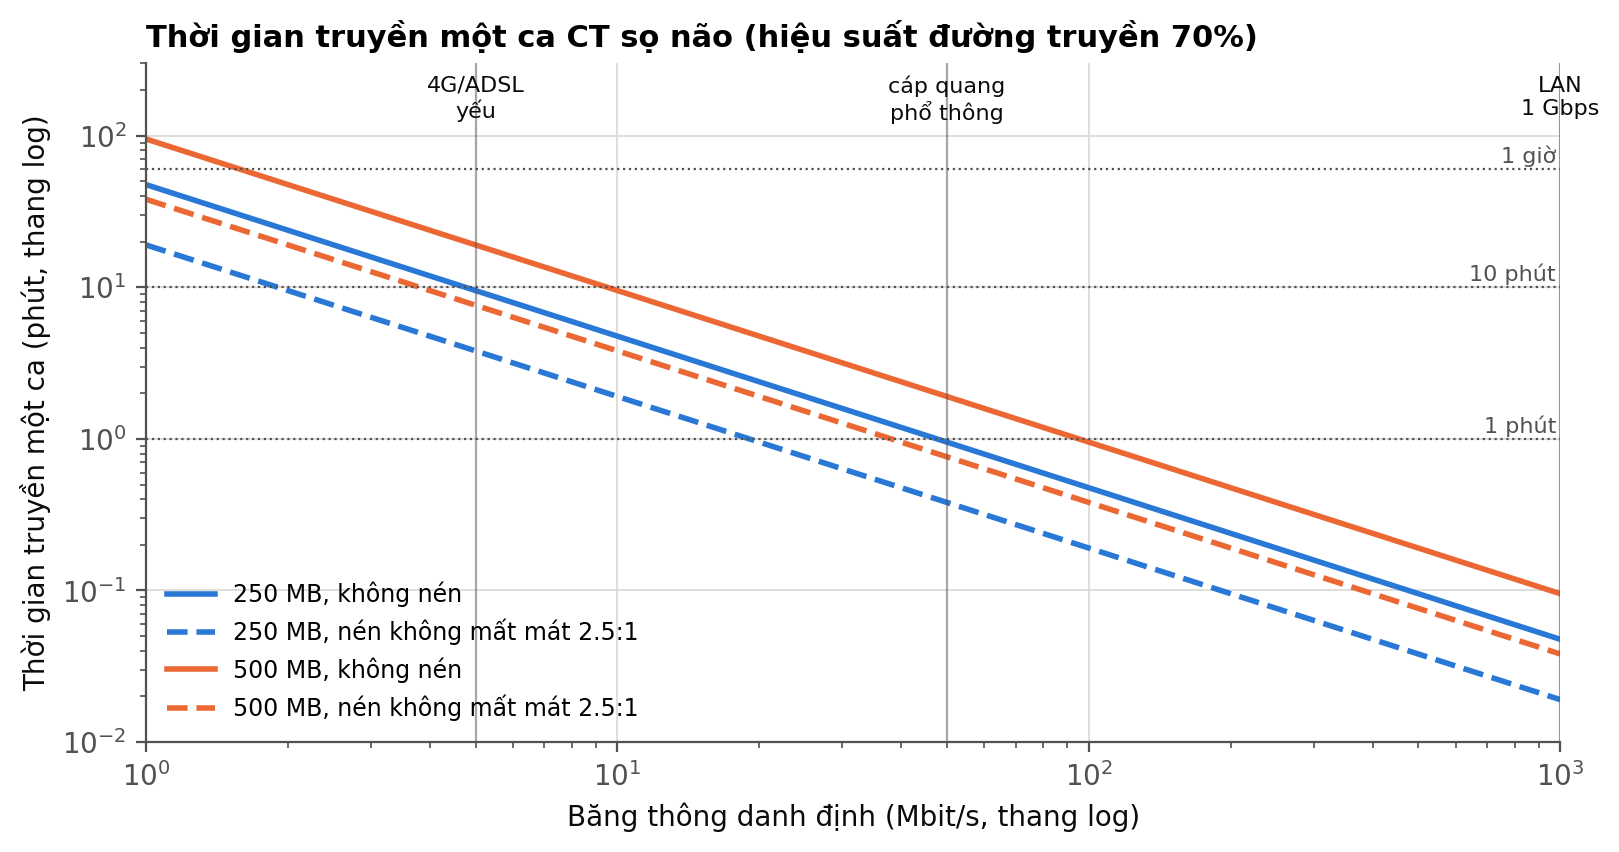
\includegraphics[width=0.88\textwidth]{figures/fig_transfer_time.png}
\caption{Ước lượng thời gian truyền một ca CT sọ não theo băng thông danh định, với
hiệu suất sử dụng đường truyền giả định 70\% và tỉ lệ nén không mất mát giả định
2{,}5:1 (nét đứt). Đây là ước lượng bậc độ lớn, không phải số đo. Mã nguồn:
\texttt{figures/src/fig\_transfer\_time.py}.}
\label{fig:transfer}
\end{figure}

\textbf{Thứ tư, tối thiểu hoá dữ liệu.} Theo yêu cầu L2, chỉ dữ liệu thực sự cần
thiết mới được truyền đi. Khử định danh và mã hoá là các bước xử lý cần thực
hiện trên bản gốc. Nếu dữ liệu được đẩy ra ngoài ngay khi vừa đến thì sẽ không
còn thời điểm nào để chèn các bước này vào giữa. Kho cục bộ tạo ra chính khoảng
thời gian đó.

\subsubsection{Yêu cầu lưu trữ bền}
\label{sec:durability}

Nguyên tắc P5 biến độ bền của kho lưu trữ thành yêu cầu chức năng. Cần phân biệt
bốn đại lượng: \emph{độ bền} (xác suất một đối tượng đã xác nhận không bị mất),
\emph{tính sẵn sàng} (tỉ lệ thời gian ảnh đọc được), \emph{RPO} (lượng dữ liệu tối
đa có thể mất, đo bằng thời gian) và \emph{RTO} (thời gian tối đa để khôi phục
dịch vụ). Một kho có thể sẵn sàng cao mà độ bền thấp, chẳng hạn một máy chủ chạy
ổn định trên một ổ đĩa duy nhất, và ngược lại. Nền tảng đạt độ bền bằng các cơ
chế chồng lớp sau, mỗi cơ chế chống lại một loại sự cố khác nhau.

\begin{enumerate}[label=D\arabic*.,leftmargin=1.2cm]
\item \textbf{Cam kết trước khi xác nhận.} Như bước B2: đối tượng được ghi
      xuống phương tiện bền và chỉ mục được cập nhật trước khi trả lời C-STORE.
      Cơ chế này chống mất dữ liệu trong khoảnh khắc chuyển giao giữa thiết bị
      chụp và nền tảng.
\item \textbf{Dự phòng phần cứng.} Trên một máy chủ đơn lẻ, đĩa được ghép
      RAID~1 hoặc RAID~6; trên cụm nhiều máy, kho đối tượng phân tán như Ceph
      \cite{weil2006ceph} hoặc MinIO nhân bản hay mã hoá xoá (erasure coding)
      dữ liệu qua nhiều nút. Cơ chế này chống hỏng đĩa hoặc hỏng một nút, nhưng
      \emph{không} phải là sao lưu: một lệnh xoá nhầm hay mã độc tống tiền sẽ
      được nhân bản ngay lập tức.
\item \textbf{Toàn vẹn.} Tổng kiểm tra của từng đối tượng được tính khi tiếp
      nhận và lưu trong chỉ mục; Orthanc hỗ trợ sẵn việc lưu MD5 cho mỗi tệp.
      Mỗi lần sao chép sang tầng khác hay ra ngoài cơ sở đều được đối chiếu
      tổng kiểm tra, và một tác vụ nền quét định kỳ toàn bộ kho để phát hiện
      hỏng dữ liệu âm thầm trên đĩa.
\item \textbf{Sao lưu theo quy tắc 3-2-1.} Ít nhất ba bản, trên hai loại
      phương tiện, trong đó một bản ở ngoài cơ sở. Bản ngoài cơ sở là bản sao
      lưu đã mã hoá ở bước B7, chống các sự cố mất toàn bộ địa điểm như cháy,
      ngập, trộm thiết bị.
\item \textbf{Bất biến.} Nhật ký truy vết và bản sao lưu ngoài cơ sở được ghi
      theo chế độ ghi một lần (WORM, hay khoá đối tượng trên kho tương thích
      S3) trong suốt thời hạn lưu trữ, để cả người vận hành lẫn mã độc đều
      không sửa hay xoá được trước hạn.
\item \textbf{Chỉ mục là dữ liệu dẫn xuất.} Vì mỗi tệp DICOM tự mô tả, mang
      đầy đủ siêu dữ liệu bên trong (Mục~\ref{sec:dicom}), kho điểm ảnh là
      nguồn dữ liệu gốc còn chỉ mục có thể dựng lại bằng cách quét lại kho. Chỉ
      mục vẫn được sao lưu (kèm nhật ký giao dịch nếu dùng PostgreSQL) để khôi
      phục nhanh, nhưng mất chỉ mục không đồng nghĩa với mất ảnh.
\item \textbf{Diễn tập khôi phục.} Việc khôi phục từ bản sao lưu được thực
      hiện thử định kỳ và đo thời gian; một bản sao lưu chưa từng được khôi phục
      thử thì chưa thể coi là bản sao lưu.
\end{enumerate}

\subsubsection{Phân tầng lưu trữ theo vòng đời}
\label{sec:tiering}

Tần suất truy cập ảnh y khoa giảm theo tuổi của ca chụp một cách khá dự đoán
được: cao trong vài tháng đầu cho việc đọc và tái khám, giảm mạnh sau 6--12 tháng
và hiếm khi được truy cập sau 2--3 năm \cite{awspacs2026}, trong khi thời hạn lưu
trữ hồ sơ bệnh án theo quy định kéo dài nhiều năm. Giữ toàn bộ dữ liệu trên
phương tiện đắt tiền nhất là lãng phí; ngược lại, đưa ca chụp của tuần trước
xuống kho lạnh sẽ làm hỏng trải nghiệm đọc ảnh. Nền tảng vì vậy chia kho thành
bốn tầng (Bảng~\ref{tab:tiers}, Hình~\ref{fig:tiers}).

\begin{table}[H]
\centering
\small
\begin{tabularx}{\textwidth}{@{}l Y Y Y p{2.3cm}@{}}
\toprule
\textbf{Tầng} & \textbf{Vị trí và phương tiện} & \textbf{Dữ liệu} & \textbf{Vai trò} & \textbf{Truy xuất} \\
\midrule
T0 -- Nóng & Tại chỗ; SSD hoặc HDD RAID gắn với cổng DICOM & Ca chụp đến 12 tháng tuổi và mọi ca đang được đọc hoặc vừa được nạp trước & Phục vụ đọc ảnh & mili giây \\
T1 -- Ấm & Tại chỗ; kho đối tượng tương thích S3 (MinIO, Ceph RGW) hoặc NAS dung lượng lớn & Ca chụp 1--3 năm tuổi & So sánh với ca cũ, tái khám & dưới 1 giây -- vài giây \\
T2 -- Ngoài cơ sở & Trung tâm dữ liệu tuyến trên hoặc đám mây đặt tại Việt Nam & Bản sao lưu mã hoá của mọi ca; bản đã khử định danh nếu bật chia sẻ & Sao lưu 3-2-1, đọc từ xa & giây -- phút qua WAN \\
T3 -- Lạnh & Ngoài cơ sở; lớp lưu trữ lạnh của kho đối tượng hoặc băng từ & Bản sao lưu của ca trên 3 năm tuổi & Lưu trữ tuân thủ thời hạn & giờ \\
\bottomrule
\end{tabularx}
\caption{Bốn tầng lưu trữ của nền tảng. Ngưỡng tuổi là giá trị mặc định, cấu hình
được theo từng cơ sở.}
\label{tab:tiers}
\end{table}

\begin{figure}[H]
\centering
\begin{tikzpicture}[
    tier/.style={draw, rounded corners=2pt, text width=7.0cm, minimum height=1.0cm,
                 align=left, font=\small, inner xsep=6pt},
    lat/.style={font=\scriptsize, align=left, text width=2.4cm},
    arr/.style={->, >=stealth, thick}
]
\node[tier, fill=red!8] (t0) {\textbf{T0 -- Nóng} (tại chỗ)\\\scriptsize SSD/HDD RAID gắn với cổng DICOM; ca $\le$ 12 tháng};
\node[tier, fill=orange!10, below=1.0cm of t0] (t1) {\textbf{T1 -- Ấm} (tại chỗ)\\\scriptsize kho đối tượng tương thích S3 hoặc NAS; 1--3 năm};
\node[tier, fill=blue!8, below=1.0cm of t1] (t2) {\textbf{T2 -- Ngoài cơ sở} (trong lãnh thổ Việt Nam)\\\scriptsize bản sao lưu mã hoá của mọi ca; bản khử định danh};
\node[tier, fill=gray!12, below=1.0cm of t2] (t3) {\textbf{T3 -- Lạnh} (ngoài cơ sở)\\\scriptsize lớp lưu trữ lạnh hoặc băng từ; $>$ 3 năm};
\node[lat, right=0.3cm of t0] {mili giây};
\node[lat, right=0.3cm of t1] {dưới 1 giây -- vài giây};
\node[lat, right=0.3cm of t2] {giây -- phút (qua WAN)};
\node[lat, right=0.3cm of t3] {giờ};
\draw[arr] ([xshift=-1.6cm]t0.south) -- node[left,font=\scriptsize] {chuyển tầng theo tuổi} ([xshift=-1.6cm]t1.north);
\draw[arr] ([xshift=1.6cm]t1.north) -- node[right,font=\scriptsize] {nạp trước ca cũ} ([xshift=1.6cm]t0.south);
\draw[arr, dashed] (t0.west) -- ++(-2.5,0) |- node[pos=0.25,left,font=\scriptsize,align=right] {sao chép\\bất đồng bộ\\(B7--B8)} (t2.west);
\draw[arr] ([xshift=-1.6cm]t2.south) -- node[left,font=\scriptsize] {chuyển tầng theo tuổi} ([xshift=-1.6cm]t3.north);
\end{tikzpicture}
\caption{Phân tầng lưu trữ. Hai tầng trên nằm tại bệnh viện và phục vụ đọc ảnh; hai
tầng dưới nằm ngoài cơ sở và phục vụ độ bền (quy tắc 3-2-1) cùng thời hạn lưu trữ.
Bên phải là thời gian truy xuất điển hình.}
\label{fig:tiers}
\end{figure}

Ba quyết định thiết kế đi kèm việc phân tầng:

\begin{itemize}
\item \textbf{Một giao diện lưu trữ cho mọi tầng.} Kho tương thích S3 được dùng
      cho cả T1 tại chỗ lẫn T2--T3 ngoài cơ sở, nên cổng DICOM chỉ cần một
      plugin lưu trữ đối tượng, và việc chuyển tầng trở thành chính sách vòng
      đời của kho chứ không phải mã nguồn riêng. Điều này phù hợp với P2: cùng
      một bản cài đặt, khác nhau ở cấu hình đích lưu trữ.
\item \textbf{Nạp trước theo chỉ định.} Khi HIS/RIS phát một chỉ định mới
      (Mục~\ref{sec:his}), bộ điều phối kéo các ca cũ của cùng bệnh nhân từ T1
      hoặc T2 lên T0 trước khi bệnh nhân được chụp, để bác sĩ so sánh được ngay
      khi ca mới đến. Đây là thực hành chuẩn của PACS và là lý do T1 phải
      truy xuất được trong vài giây chứ không phải vài giờ.
\item \textbf{Xoá có căn cứ.} Khi một ca hết thời hạn lưu trữ theo L6, việc xoá
      được thực hiện đồng thời ở mọi tầng, được ghi vào nhật ký truy vết, và
      không áp dụng cho các ca đang bị giữ lại vì lý do pháp lý.
\end{itemize}

Hình~\ref{fig:storage} ước lượng quy mô dữ liệu, chỉ tính riêng CT sọ não với
100~MB mỗi ca sau khi nén không mất mát. Một cơ sở bối cảnh A với khoảng 60 ca
mỗi ngày tích luỹ khoảng 2{,}2~TB mỗi năm, bối cảnh B với khoảng 30 ca mỗi ngày
khoảng 1{,}1~TB mỗi năm, và bối cảnh C với khoảng 5 ca mỗi ngày chỉ khoảng
0{,}18~TB mỗi năm. Điểm quan trọng là tầng nóng T0 \emph{không} tăng theo thời
gian: nó dừng ở mức một năm dữ liệu, trong khi toàn bộ phần tăng trưởng dồn vào
các tầng rẻ hơn. Toàn bộ khoa chẩn đoán hình ảnh, gồm các vùng chụp khác, MRI và
X-quang, sẽ lớn hơn nhiều lần; con số cần được tính lại theo thống kê thực tế của
từng cơ sở khi triển khai.

\begin{figure}[H]
\centering
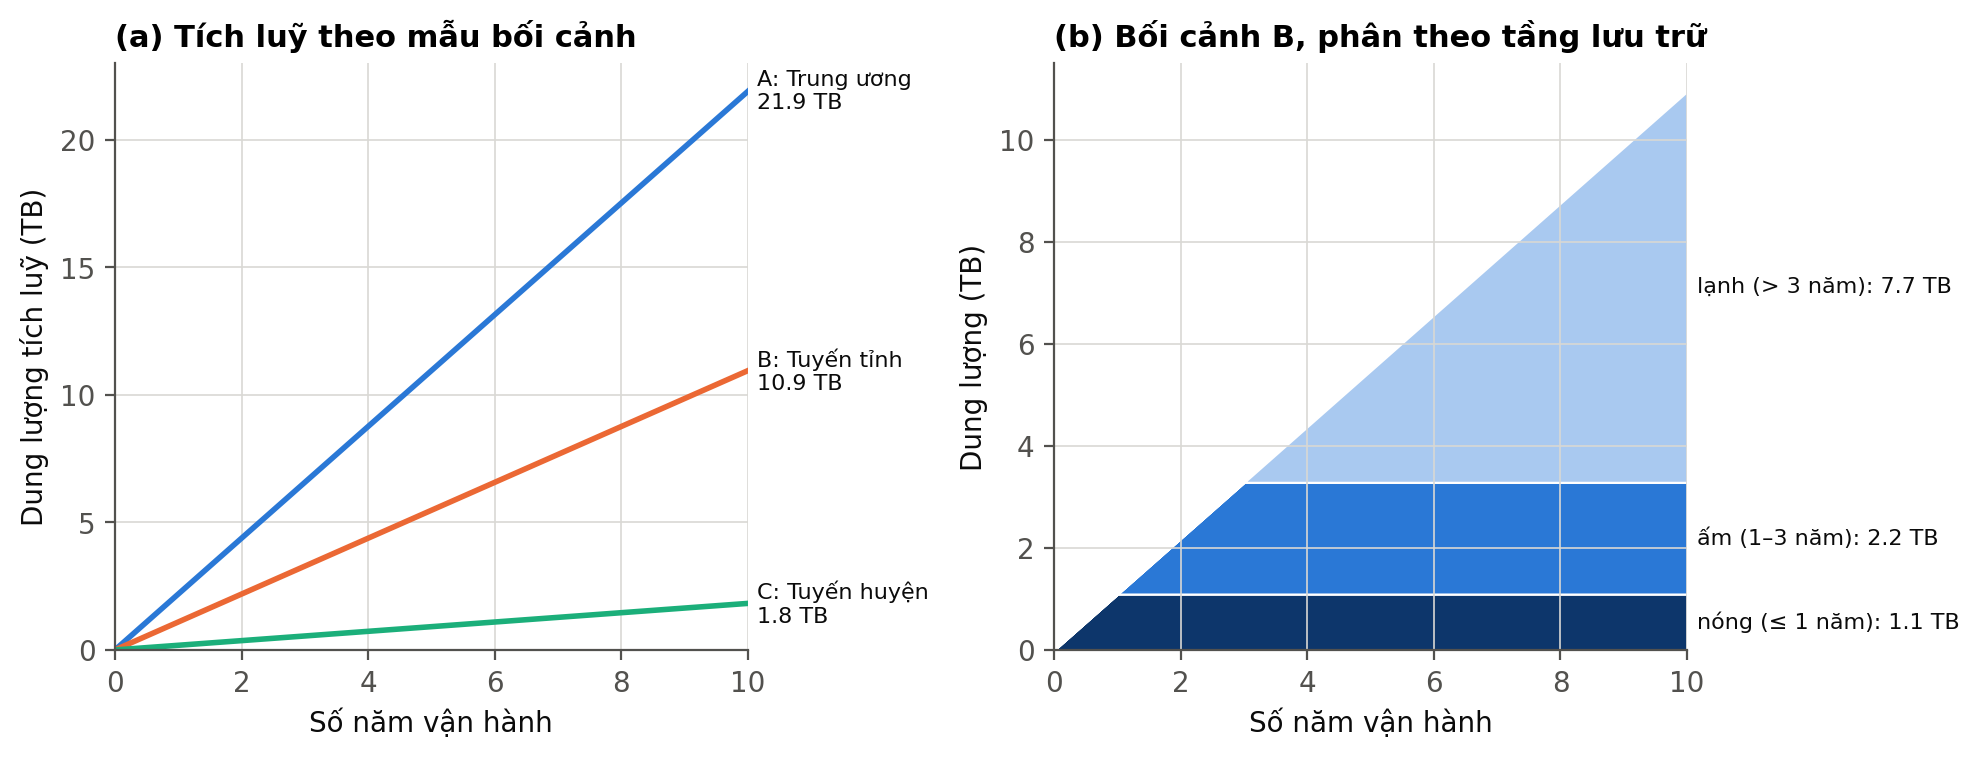
\includegraphics[width=\textwidth]{figures/fig_storage_growth.png}
\caption{Ước lượng dung lượng lưu trữ CT sọ não: (a) tích luỹ theo mẫu bối cảnh;
(b) bối cảnh B phân theo tầng lưu trữ. Giả định 250~MB/ca, nén không mất mát
2{,}5:1, ngưỡng tầng 1 và 3 năm. Mã nguồn: \texttt{figures/src/fig\_storage\_growth.py}.}
\label{fig:storage}
\end{figure}

\subsubsection{Vai trò của kho ngoài cơ sở}
\label{sec:offsite}

Kho ngoài cơ sở không tham gia vào việc cung cấp hình ảnh cho bác sĩ đọc tại
chỗ. Nó phục vụ ba mục đích, mỗi mục đích nhận một loại bản sao khác nhau:

\begin{enumerate}
\item \textbf{Sao lưu và lưu trữ dài hạn.} Nhận bản sao lưu của bản gốc, được
      mã hoá trước khi rời bệnh viện bằng khoá do bệnh viện quản lý, nên bên
      vận hành kho ngoài cơ sở chỉ giữ dữ liệu đã mã hoá. Để tránh hoàn toàn
      câu hỏi về chuyển dữ liệu xuyên biên giới, kho này được đặt trong lãnh
      thổ Việt Nam và được ràng buộc bằng hợp đồng xử lý dữ liệu.
\item \textbf{Chẩn đoán hình ảnh từ xa.} Nhận bản đã khử định danh để bác sĩ
      tuyến trên đọc (Mục~\ref{sec:percontext}, bối cảnh C). Bảng ánh xạ từ
      định danh giả về định danh thật chỉ nằm tại cơ sở gửi, nên kết quả đọc
      trả về được gắn lại đúng bệnh nhân tại chỗ.
\item \textbf{Tích luỹ dữ liệu phục vụ nghiên cứu.} Dữ liệu đã khử định danh
      kèm kết quả đọc của bác sĩ tạo thành tập dữ liệu phục vụ các nghiên cứu
      về sau. Theo yêu cầu L7, mục đích này phải có căn cứ pháp lý riêng,
      tách bạch với mục đích khám chữa bệnh.
\end{enumerate}

Không mục đích nào trong ba mục đích trên mang tính cấp thời, nên kho ngoài cơ sở
có thể ngừng hoạt động mà hệ thống vẫn phục vụ đầy đủ chức năng lâm sàng: đây là
thuộc tính thiết kế quan trọng nhất của mô hình lưu trữ này. Tuy nhiên, \emph{chức
năng} không phụ thuộc vào kho ngoài cơ sở không có nghĩa là \emph{độ bền} không phụ
thuộc: ở nơi chỉ có một máy chủ, bản sao lưu ngoài cơ sở là lớp bảo vệ duy nhất
trước sự cố mất toàn bộ địa điểm (D4).

\begin{table}[H]
\centering
\small
\begin{tabularx}{\textwidth}{@{}l Y Y Y@{}}
\toprule
\textbf{Tiêu chí} & \textbf{Kho tại chỗ (T0--T1)} & \textbf{Sao lưu ngoài cơ sở (T2--T3)} & \textbf{Bản chia sẻ (T2)} \\
\midrule
Dữ liệu & Bản gốc còn định danh & Bản gốc, đã mã hoá & Bản đã khử định danh \\
Tính bắt buộc & Bắt buộc & Khuyến nghị; bắt buộc nếu chỉ có một máy chủ & Tuỳ chọn, mặc định tắt \\
Thời điểm ghi & Đồng bộ, trước khi xác nhận & Bất đồng bộ, sau B6 & Bất đồng bộ, sau B6 \\
Khi mất mạng & Không ảnh hưởng & Hàng đợi dài thêm, không mất dữ liệu & Hàng đợi dài thêm \\
Vai trò trong đọc ảnh & Nguồn dữ liệu chính & Chỉ dùng khi khôi phục & Đọc từ xa \\
Ràng buộc pháp lý & Thuộc phạm vi bệnh viện & Đặt tại Việt Nam, hợp đồng xử lý dữ liệu & Khử định danh theo PS3.15; mục đích L7 \\
\bottomrule
\end{tabularx}
\caption{Phân vai giữa kho tại chỗ và hai loại bản sao ngoài cơ sở.}
\label{tab:localcloud}
\end{table}

\subsection{Áp dụng vào từng bối cảnh bệnh viện}
\label{sec:percontext}

Mỗi kiến trúc dưới đây là một cấu hình của mô hình chung, được mô tả theo cùng
một khung: hiện trạng của cơ sở, cách triển khai, cách hiện thực các tầng lưu
trữ, kết nối và đồng bộ, và hành vi khi có sự cố.

\subsubsection{Kiến trúc A: bệnh viện tuyến trung ương, tích hợp dạng đi kèm}

\textbf{Hiện trạng.} Cơ sở đã có PACS hoặc VNA thương mại vận hành ổn định, có
sao lưu, tích hợp với HIS/RIS qua HL7, có phòng CNTT và mạng nội bộ dự phòng.
Khối lượng trên 50 ca CT sọ não mỗi ngày, bác sĩ chẩn đoán hình ảnh trực 24/7.
Yêu cầu là không làm xáo trộn quy trình và không thay thế hệ thống sẵn có.

\textbf{Triển khai.} Cổng DICOM được triển khai không phải như kho lưu trữ mà
như một thành phần \emph{đi kèm} (sidecar): PACS được cấu hình để chuyển tiếp các
ca chụp CT sọ não tới nó bằng luật định tuyến C-STORE, và nền tảng ghi kết quả
xử lý ngược trở lại dưới dạng đối tượng DICOM Structured Report hoặc Secondary
Capture, hoặc thông qua giao diện danh sách chờ đọc của nhà cung cấp nếu có.
Để đáp ứng thông lượng, dịch vụ xử lý hậu kỳ phi trạng thái được nhân bản theo
chiều ngang, và nhiều phiên bản cổng DICOM dùng chung một chỉ mục PostgreSQL và
một kho đối tượng.

\textbf{Lưu trữ.} PACS sẵn có là nguồn dữ liệu gốc và tự đảm nhận T1--T3 cùng
sao lưu. Nền tảng chỉ giữ một bộ đệm T0 cuốn chiếu, chẳng hạn 90 ngày, tương
đương khoảng 0{,}55~TB với khối lượng trên, cộng với các kết quả do nó sinh ra;
các kết quả này được ghi ngược về PACS nên cũng được PACS lưu trữ dài hạn. Vì
vậy yêu cầu độ bền với nền tảng ở bối cảnh này nhẹ hơn hẳn: mất bộ đệm chỉ cần
lấy lại từ PACS bằng C-MOVE. Nguyên tắc chung là trách nhiệm về độ bền thuộc về
nơi giữ bản gốc.

\textbf{Kết nối.} Chỉ mạng nội bộ; không có đích ngoài cơ sở.

\textbf{Khi có sự cố.} Tính chất cốt yếu là gỡ bỏ nền tảng sẽ đưa bệnh viện trở
lại đúng trạng thái trước đó: không một thành phần sẵn có nào phụ thuộc vào nó.
Nếu nền tảng ngừng hoạt động, luật chuyển tiếp của PACS xếp hàng và gửi lại khi
nền tảng hoạt động trở lại.

\subsubsection{Kiến trúc B: bệnh viện tuyến tỉnh, triển khai tích hợp}

\textbf{Hiện trạng.} Có PACS nhưng có thể là sản phẩm đời cũ, dung lượng hạn
chế, hỗ trợ DICOMweb không chắc chắn. Có một đến hai nhân sự CNTT đa năng và một
số máy chủ; GPU chưa chắc có. Khối lượng 10--50 ca CT sọ não mỗi ngày; bác sĩ chẩn
đoán hình ảnh chỉ có mặt trong giờ hành chính. Đây là trường hợp phổ biến nhất và
là mục tiêu chính.

\textbf{Triển khai.} Nền tảng cung cấp cả cổng DICOM lẫn trình xem, hoạt động
song song với PACS. Khi PACS hỗ trợ DICOMweb, nền tảng đọc dữ liệu từ đó; khi
không, thiết bị chụp được cấu hình gửi đồng thời tới cả PACS và cổng DICOM, việc
trùng lặp này được ưu tiên hơn so với phụ thuộc vào một giao diện có thể không
hoạt động. Toàn bộ dịch vụ đóng gói container trên một đến hai máy chủ, đặt sau
reverse proxy đảm nhiệm kết thúc TLS và chuyển tiếp các yêu cầu DICOMweb. Đây là
cấu hình mà bản mẫu hiện tại hiện thực.

\textbf{Lưu trữ.} Nền tảng giữ bản gốc của riêng nó và hiện thực đủ bốn tầng.
T0 là mảng RAID trên máy chủ cổng DICOM, giữ khoảng một năm dữ liệu, tức cỡ
1{,}1~TB cho CT sọ não. T1 là kho đối tượng tương thích S3 tại chỗ, trên ba nút
trở lên nếu có đủ máy chủ, hoặc một NAS RAID~6 nếu không; sau mười năm, phần này
chứa phần lớn trong khoảng 11~TB tích luỹ (Hình~\ref{fig:storage}b). T2--T3 là
bản sao lưu mã hoá gửi tới trung tâm dữ liệu của tuyến trung ương hoặc một dịch
vụ đám mây đặt tại Việt Nam. Với chỉ một đến hai nhân sự CNTT, sao lưu, quét toàn
vẹn và diễn tập khôi phục phải được tự động hoá hoàn toàn và báo cáo qua giám sát
chứ không dựa vào thao tác thủ công.

\textbf{Kết nối.} Đọc ảnh trong giờ hành chính qua mạng nội bộ. Ngoài giờ, bác sĩ
trực từ xa truy cập trình xem qua VPN hoặc qua reverse proxy có xác thực; với
đường truyền 50~Mbps, một ca 250~MB cần khoảng một phút (Hình~\ref{fig:transfer}),
và cơ chế tải lũy tiến (Mục~\ref{sec:transfersyntax}) cho phép bắt đầu đọc sớm
hơn nữa. Cơ sở tuyến tỉnh cũng là ứng viên tự nhiên để làm trung tâm cho các cơ
sở tuyến huyện trong tỉnh (Mục~\ref{sec:hub}).

\textbf{Khi có sự cố.} Hỏng một đĩa: RAID che giấu, không gián đoạn. Hỏng máy chủ
cổng DICOM: PACS vẫn nhận ảnh nhờ gửi song song; nền tảng được dựng lại và khôi
phục từ T1 hoặc T2 trong vài giờ. Mất Internet: đọc tại chỗ không ảnh hưởng, chỉ
hàng đợi sao lưu dài thêm và đọc từ xa ngoài giờ bị gián đoạn.

\subsubsection{Kiến trúc C: bệnh viện tuyến huyện, thiết bị trọn gói}

\textbf{Hiện trạng.} Có máy CT nhưng không có PACS; hình ảnh nằm trên ổ cứng của
máy trạm thiết bị chụp, dung lượng có hạn và thường bị ghi đè khi đầy, nên rủi ro
mất ảnh là tình trạng sẵn có chứ không phải rủi ro mới. Không có phòng máy chủ,
không có nhân sự CNTT, không có bác sĩ chẩn đoán hình ảnh tại chỗ; nguồn điện và
kết nối mạng có thể không ổn định. Khối lượng dưới 10 ca CT sọ não mỗi ngày.

\textbf{Triển khai.} Nền tảng được chuyển giao dưới dạng một thiết bị trọn gói đã
cấu hình sẵn: một máy duy nhất, các dịch vụ đóng gói container, bộ lưu điện kèm
cơ chế tắt máy an toàn, quy trình lắp đặt chỉ gồm kết nối vật lý và một thay đổi
cấu hình trên thiết bị chụp. Cổng DICOM đóng luôn vai trò PACS của bệnh viện. Thiết
bị tự giám sát và gửi cảnh báo (đĩa, dung lượng, độ dài hàng đợi, nhiệt độ) tới đơn
vị hỗ trợ ở tuyến trên, vì tại chỗ không có ai đọc được bảng giám sát.

\textbf{Lưu trữ.} T0 và T1 gộp làm một trên thiết bị: hai ổ đĩa ghép RAID~1. Với
khoảng 0{,}18~TB CT sọ não mỗi năm, hai ổ vài TB đủ cho nhiều năm; con số cần được
tính lại theo tổng số ca của khoa. Vì chỉ có một thiết bị tại một địa điểm, bản sao
lưu mã hoá ngoài cơ sở (T2), đặt tại cơ sở tuyến tỉnh làm trung tâm, là lớp bảo vệ
duy nhất trước việc mất toàn bộ thiết bị; ở bối cảnh này nó là bắt buộc chứ không
còn là khuyến nghị.

\textbf{Kết nối và đồng bộ.} Toàn bộ chức năng tiếp nhận, lưu trữ và hiển thị chạy
cục bộ, nên mất kết nối không làm vô hiệu hoá hệ thống. Liên kết với tuyến trên là
\emph{theo cơ hội}: khi có kết nối, hàng đợi được giải phóng dần theo khả năng của
đường truyền. Trên đường truyền 5~Mbps, một ca 250~MB đã nén cần khoảng bốn phút
(Hình~\ref{fig:transfer}), nên hàng đợi cần phân mức ưu tiên: ca được đánh dấu
cần đọc từ xa đi trước, bản sao lưu đi sau và được giới hạn băng thông trong giờ
cao điểm. Bản gửi đọc từ xa là bản đã khử định danh; bảng ánh xạ định danh giả
nằm trên thiết bị, nên kết quả đọc trả về được gắn lại đúng bệnh nhân tại chỗ.

\textbf{Khi có sự cố.} Mất mạng: hàng đợi dài thêm, không mất dữ liệu. Hỏng một
đĩa: RAID~1 che giấu, thiết bị cảnh báo để thay đĩa. Mất điện: bộ lưu điện cho
phép tắt máy an toàn, và nhờ nguyên tắc P5 thiết bị chụp sẽ gửi lại các lát cắt
chưa được xác nhận. Mất toàn bộ thiết bị: thay thiết bị mới và khôi phục từ bản
sao lưu tại tuyến trên; RPO bằng độ trễ của hàng đợi sao lưu tại thời điểm sự cố.

Vì không có bác sĩ chẩn đoán hình ảnh tại chỗ, giá trị chính của cấu hình này nằm
ở hai điểm: không còn mất ảnh do máy trạm bị ghi đè, và rút ngắn thời gian đưa hình
ảnh tới người đọc có chuyên môn ở tuyến trên, thay vì chờ chuyển bệnh nhân hoặc
chuyển dữ liệu thủ công qua đĩa quang.

\subsubsection{So sánh}

\begin{table}[H]
\centering
\small
\begin{tabularx}{\textwidth}{@{}l Y Y Y@{}}
\toprule
& \textbf{A: Đi kèm} & \textbf{B: Tích hợp} & \textbf{C: Trọn gói} \\
\midrule
Nguồn dữ liệu gốc & PACS sẵn có & Nền tảng, song song PACS & Nền tảng \\
Tầng T0 & Bộ đệm cuốn chiếu $\sim$90 ngày & RAID trên máy chủ, $\sim$1 năm & RAID~1 trên thiết bị (gộp T0--T1) \\
Tầng T1 & Do PACS đảm nhận & Kho đối tượng S3 hoặc NAS tại chỗ & Gộp vào T0 \\
Tầng T2--T3 & Do PACS đảm nhận & Sao lưu mã hoá tới tuyến trên hoặc đám mây trong nước & Sao lưu mã hoá tới trung tâm tuyến tỉnh (bắt buộc) \\
Dung lượng CT sọ não & $\sim$2{,}2~TB/năm & $\sim$1{,}1~TB/năm & $\sim$0{,}18~TB/năm \\
Trình xem & Sẵn có & Nền tảng (OHIF) & Nền tảng (OHIF) \\
Trả kết quả & DICOM SR về PACS & Hiển thị trên trình xem & Trình xem + kết quả đọc từ xa \\
Phụ thuộc mạng & Chỉ mạng nội bộ & Mạng nội bộ; Internet cho đọc ngoài giờ & Chịu được mất kết nối \\
Hỏng máy chủ & Không ảnh hưởng lâm sàng & Khôi phục trong vài giờ từ T1/T2 & Thay thiết bị, khôi phục từ tuyến trên \\
Vai trò lâm sàng & Bổ trợ quy trình sẵn có & Hỗ trợ ngoài giờ & Lưu trữ an toàn, kết nối tuyến trên \\
\bottomrule
\end{tabularx}
\caption{So sánh ba kiến trúc được đề xuất.}
\label{tab:arch}
\end{table}

\subsection{Mở rộng liên viện: mô hình trục--nan}
\label{sec:hub}

Khi nhiều cơ sở tuyến huyện cùng gửi ca chụp lên một cơ sở tuyến trên, các kiến
trúc C riêng lẻ ghép lại thành mô hình trục--nan (hub-and-spoke), tương tự kiến
trúc PACS lai mà AWS đề xuất cho các mạng lưới nhiều bệnh viện \cite{awspacs2026}:
mỗi cơ sở giữ kho cục bộ và phục vụ đọc tại chỗ ở tốc độ mạng nội bộ, còn trung
tâm nhận bản sao bất đồng bộ và giữ một chỉ mục chung chỉ chứa siêu dữ liệu (ca
chụp nào đang nằm ở cơ sở nào, ở tầng nào, đã đồng bộ tới đâu), không chứa dữ liệu
điểm ảnh.

\begin{figure}[H]
\centering
\begin{tikzpicture}[
    site/.style={draw, rounded corners=2pt, align=center, font=\small,
                 minimum width=3.0cm, minimum height=1.1cm, fill=green!6},
    hubbox/.style={draw, rounded corners=3pt, align=left, font=\small,
                   fill=blue!6, text width=6.6cm, inner sep=6pt},
    arr/.style={->, >=stealth, thick},
    sync/.style={->, >=stealth, thick, dashed}
]
\node[hubbox] (hub) {\textbf{Trung tâm}: bệnh viện tuyến tỉnh hoặc trung tâm dữ liệu trong nước\\[2pt]
  \scriptsize $\bullet$ chỉ mục vị trí ca chụp (chỉ siêu dữ liệu)\\
  \scriptsize $\bullet$ kho sao lưu mã hoá (T2--T3) của các cơ sở\\
  \scriptsize $\bullet$ kho ca chụp đã khử định danh chờ đọc từ xa\\
  \scriptsize $\bullet$ trình xem cho bác sĩ đọc từ xa};
\node[site, fill=orange!8, above=1.1cm of hub] (a) {Bệnh viện tuyến trung ương\\\scriptsize hội chẩn khi cần};
\node[site, below left=1.5cm and 0.6cm of hub] (c1) {Cơ sở C$_1$\\\scriptsize thiết bị trọn gói};
\node[site, below=1.5cm of hub] (c2) {Cơ sở C$_2$\\\scriptsize thiết bị trọn gói};
\node[site, below right=1.5cm and 0.6cm of hub] (c3) {Cơ sở C$_3$\\\scriptsize thiết bị trọn gói};
\foreach \c in {c1, c2, c3} {
  \draw[sync] (\c) to[bend left=12] (hub);
  \draw[arr] (hub) to[bend left=12] (\c);
}
\draw[sync] (hub) -- node[right,font=\scriptsize] {ca cần hội chẩn} (a);
\end{tikzpicture}
\caption{Mô hình trục--nan. Nét đứt: dữ liệu đi lên, bất đồng bộ qua hàng đợi (bản sao
lưu mã hoá và bản đã khử định danh). Nét liền: kết quả đọc trả về cơ sở dưới dạng
DICOM SR và được gắn lại định danh tại chỗ.}
\label{fig:hubspoke}
\end{figure}

Mô hình này tiếp thu ba điểm từ kiến trúc tham chiếu của AWS: tách chỉ mục khỏi
điểm ảnh, sao chép bất đồng bộ không chặn luồng lâm sàng, và phân tầng lưu trữ tại
trung tâm theo vòng đời. Nó khác ở ba giả định. Thứ nhất, trung tâm đặt tại hạ tầng
trong nước, không đặt tại một vùng đám mây ở nước ngoài, theo L1. Thứ hai, kết nối
giữa cơ sở và trung tâm là đường Internet không ổn định chứ không phải kênh riêng,
nên mọi tương tác đều bất đồng bộ và cơ sở không bao giờ phải chờ trung tâm. Thứ ba,
trung tâm chỉ thấy bản sao lưu đã mã hoá và bản đã khử định danh; do đó nó chưa có
chỉ mục bệnh nhân chung (MPI) liên kết các ca của cùng một người ở nhiều cơ sở. Việc
liên kết đó đòi hỏi xử lý dữ liệu định danh ở trung tâm, chẳng hạn dựa trên số định
danh cá nhân khi hồ sơ bệnh án điện tử đã kết nối cơ sở dữ liệu quốc gia về dân cư,
và cần căn cứ pháp lý riêng; đây là câu hỏi mở cho các giai đoạn sau.

\subsection{Bản mẫu}

Một bản mẫu hiện thực Kiến trúc B đã được xây dựng nhằm kiểm chứng mô hình thành
phần. Bản mẫu gồm các dịch vụ đóng gói container: Orthanc mở cổng DICOM cổ điển
để nhận dữ liệu từ thiết bị chụp và DICOMweb cho trình xem; OHIF chạy sau một
reverse proxy chuyển tiếp \texttt{/dicom-web} và \texttt{/wado} tới Orthanc, nhờ
đó tránh được các vấn đề về cross-origin; và một dịch vụ xử lý hậu kỳ được gọi
bởi callback Lua của Orthanc kích hoạt khi đối tượng ảnh đến.

Bản mẫu xác nhận cơ chế kích hoạt theo sự kiện và hướng tích hợp với trình xem.
Nó \emph{chưa} sẵn sàng triển khai: xác thực bị tắt và kênh truyền chưa được mã
hoá. Mỗi điểm trong số đó tương ứng với một yêu cầu ở Mục~\ref{sec:legal} và
được lên lịch xử lý trong Giai đoạn~2, cùng với các tầng T1--T3, hàng đợi đồng bộ
và các cơ chế độ bền D3--D7.

\subsection{Kiến trúc an toàn thông tin}

Việc hiện thực các yêu cầu ở Mục~\ref{sec:legal} đòi hỏi: kết thúc TLS tại
reverse proxy, với DICOM cổ điển được giới hạn trong một phân đoạn mạng riêng
hoặc bọc trong đường hầm, và xác thực nút mạng theo hồ sơ IHE ATNA khi DICOM đi qua
mạng không tin cậy \cite{iheiti}; xác thực người dùng qua một máy chủ định danh
OpenID Connect như Keycloak, liên kết với hệ thống thư mục của bệnh viện nếu có,
và phân quyền cho Orthanc qua plugin phân quyền nâng cao cùng orthanc-auth-service
\cite{keycloak,orthancauth}, kèm phân tách vai trò giữa bác sĩ chẩn đoán hình ảnh,
bác sĩ chỉ định và quản trị viên; mã hoá khi lưu trữ cho cả kho ảnh lẫn kho siêu
dữ liệu, với khoá mã hoá bản sao lưu ngoài cơ sở do bệnh viện nắm giữ; nhật ký truy
vết chỉ ghi thêm cho mọi lượt truy cập, lưu giữ theo L6; và khử định danh áp dụng
tại ranh giới của bộ điều phối, để các thuộc tính định danh không bao giờ rời khỏi
phạm vi kiểm soát. Việc cho phép truy cập ẩn danh và truyền dữ liệu ở dạng rõ
trong bản mẫu là những tiện lợi phục vụ phát triển, và bị cấm khi triển khai thực
tế.


\newpage
\section{Kết luận và kế hoạch Giai đoạn 2}

\subsection{Tổng kết}

Giai đoạn~1 đã thiết lập nền móng cho một nền tảng phần mềm quản lý và khai thác
dữ liệu ảnh y khoa phục vụ chẩn đoán xuất huyết não trong các bối cảnh bệnh viện
khác nhau. Kiến thức lâm sàng nền tảng đã được khảo sát, qua đó làm rõ các yêu
cầu mà quy trình đọc ảnh đặt ra cho hệ thống lưu trữ, đặc biệt là việc phải bảo
toàn dữ liệu điểm ảnh gốc để bác sĩ có thể tuỳ ý chuyển đổi cửa sổ hiển thị khi
đọc.

Chuẩn DICOM đã được trình bày như một ràng buộc kiến trúc chứ không phải một chi
tiết cài đặt: nó quy định cách dữ liệu được tiếp nhận, những thuộc tính phải
được bảo toàn để hiển thị chính xác, và những thuộc tính phải được loại bỏ trước
khi chia sẻ. Các giải pháp phần mềm hiện có đã được khảo sát và phân tích, cho
thấy một khoảng trống rõ ràng giữa các hệ thống thương mại hoàn chỉnh nhưng đắt
đỏ và khép kín, với các thành phần mã nguồn mở tuy miễn phí nhưng đòi hỏi công
sức tích hợp đáng kể.

Khung pháp lý Việt Nam, chủ yếu là Luật Bảo vệ dữ liệu cá nhân năm 2025 (kế thừa
và thay thế Nghị định 13/2023/NĐ-CP), Luật Khám bệnh, chữa bệnh và Thông tư
13/2025/TT-BYT về hồ sơ bệnh án điện tử, xác lập dữ liệu sức khoẻ là dữ liệu cá nhân nhạy cảm và điều
chỉnh việc chuyển dữ liệu ra nước ngoài chặt chẽ tới mức mô hình lưu trữ cục bộ
trước, đồng bộ đám mây sau trở thành lựa chọn mặc định hợp lý chứ không đơn
thuần là một ưu tiên thận trọng.

Một mô hình chung đã được xây dựng trước khi đi vào từng bệnh viện: luồng xử lý
chín bước của một ca chụp, nguyên tắc ghi cục bộ trước, các cơ chế độ bền D1--D7
bảo đảm ca chụp đã xác nhận không bị mất, và bốn tầng lưu trữ từ kho nóng tại chỗ
tới kho lạnh ngoài cơ sở. Ba mẫu bối cảnh bệnh viện đã được đặc tả, và ba kiến trúc
tương ứng được đề xuất như các cấu hình của mô hình chung đó, khác nhau ở nơi giữ
bản gốc, cách hiện thực các tầng lưu trữ và hành vi khi có sự cố; mô hình liên viện
trục--nan mở rộng kiến trúc C cho một mạng lưới cơ sở tuyến huyện. Kiến trúc B đã
được kiểm chứng bằng bản mẫu cho phần tiếp nhận, hiển thị và kích hoạt theo sự kiện.

\subsection{Giai đoạn 2}

\begin{enumerate}
    \item \textbf{Hoàn thiện nền tảng.} Hiện thực bộ điều phối kèm khử định
          danh, cơ chế thử lại và kiểm soát tải; hoàn thiện hàng đợi đồng bộ bền
vững mô tả tại Mục~\ref{sec:flow}.
\item \textbf{Lưu trữ bền và phân tầng.} Hiện thực các tầng T1--T3 trên kho
      tương thích S3, chính sách vòng đời và nạp trước ca cũ, cùng các cơ chế
      D3--D7 (kiểm tra toàn vẹn định kỳ, sao lưu 3-2-1 mã hoá, khoá ghi một lần,
      diễn tập khôi phục) theo Mục~\ref{sec:durability} và Mục~\ref{sec:tiering}.
\item \textbf{Tích hợp HIS/RIS.} Nhận chỉ định qua HL7 v2 hoặc FHIR, cung cấp
      Modality Worklist khi có thể, và chức năng đối chiếu định danh theo tinh
      thần IHE PIR (Mục~\ref{sec:his}).
    \item \textbf{An toàn thông tin.} Bổ sung xác thực và phân quyền theo vai
          trò, mã hoá kênh truyền và dữ liệu lưu trữ, nhật ký truy vết chỉ ghi
          thêm, theo đúng các yêu cầu tại Mục~\ref{sec:legal}.
    \item \textbf{Hoàn thiện giao diện đọc ảnh.} Tuỳ biến trình xem cho phù hợp
          với quy trình đọc ảnh sọ não, bao gồm các cửa sổ hiển thị đặt sẵn mô
          tả tại Mục~\ref{sec:windowing}.
    \item \textbf{Đánh giá.} Đo thời gian truyền thực tế và lợi ích của nén không mất
      mát, tải lũy tiến HTJ2K trên đường truyền chậm để thay các ước lượng ở
      Hình~\ref{fig:transfer}; đo RPO và RTO thực tế qua diễn tập sự cố; đo độ trễ đầu-cuối từ lúc thiết bị gửi ảnh tới lúc
          bác sĩ xem được, đo thông lượng, và đặc tả hành vi hệ thống dưới các
          kịch bản lỗi mà nguyên tắc~P1 hướng tới kiểm soát, đặc biệt là kịch
          bản mất kết nối kéo dài.
    \item \textbf{Triển khai thử nghiệm.} Với điều kiện có thoả thuận hợp tác
          phù hợp, triển khai thử tại một cơ sở y tế nhằm kiểm chứng giả định về
          hạ tầng và quy trình đã nêu ở Mục~\ref{sec:contexts}.
\end{enumerate}

Rủi ro chính đối với Giai đoạn~2 là khả năng tiếp cận một cơ sở y tế thực tế để
triển khai thử nghiệm, yếu tố mà việc kiểm chứng các giả định kiến trúc phụ
thuộc vào. Vì vậy, việc kết nối với các cơ sở y tế cần được bắt đầu sớm, và kế
hoạch đánh giá cần được xây dựng sao cho có thể chuyển về phương án kiểm thử
trên dữ liệu mô phỏng nếu không thu xếp được triển khai thực tế.


\newpage
\addcontentsline{toc}{section}{Tài liệu tham khảo}
\nocite{*}
\bibliography{refs}

\end{document}



